\input{Formato/formato}

\instituto{Universidad Tecnológica Nacional\\Facultad Regional Córdoba}
\carrera{Ingeniería Electrónica}
\catedra{}
\curso{XRX}
\title{XXXXXXX}
\subtitledoc{XXXXXXX}
\professor{
    XXXXXXXXX
    \par
    XXXXXXXXX
}

\author{
        Arenas, Nicolás
        \par
        XXXXXXXX

}
\legajo{
        86607
        \par
        XXXXX
}
\footerauthor{Arenas,XXXXX}
\footerlegajo{86607, XXXXX}
\date{\the\year}





\begin{document}
\maketitle
\tableofcontents
\newpage
\addcontentsline{toc}{chapter}{Introduccion}
E aquí la guía definitiva para comprender análisis señales y sistemas.Cabe aclarar que este es un apunte realizado por una alumno, por lo tanto, puede que tenga errores. Además de que no es un apunte oficial de la cátedra. 
En este apunte se intentara traer conceptos abstractos de manera mas visual e intuitiva para generar familiaridad con los conceptos vistos en clase.

%\chapter{Números complejos}
\unsection{Introducción}
Este es el primer tema de la materia, los números complejos nos van ayudar en el análisis de señales y sistemas por ende es de vital importancia entenderlos plenamente.
La unidad compleja se define como:
\begin{equation}\label{eq:j}
    i=\sqrt{-1}
\end{equation}{}
De esta definición podemos intuir que:
\begin{equation}\label{eq:jj}
    i^2=-1 \lrah \sqrt{-1}\cdot\sqrt{-1}=-1 
\end{equation}{}
Ahora bien, todo estudiante de ingeniería electrónica sabe que $i$ es por corriente asi que para los propositos de este curso usaremos $j$ en vez de $i$ 
\unsection{Números complejos}
Un numero complejo se puede interpretar como un vector de 2 dimensiones conformado por 2 partes, la parte real y la parte imaginaria. La unidad de la parte imaginaria sera $j$ y la unidad de la parte real sera el $1$, escalando (multiplicando por un escalar) y sumando estas 2 unidades seremos capaz de representar cualquier numero complejo, por lo tanto estas dos unidades son la base de un espacio vectorial ya que cualquier numero complejo, que es un vector, se puede expresar como la suma de estos 2 versores:
\begin{equation}\label{eq:cart}
    z=u\cdot(1,j0)+v\cdot (0,j1)
\end{equation}
Siendo $u$ y $v$ números reales.
\begin{figure}[H]
    \centering
         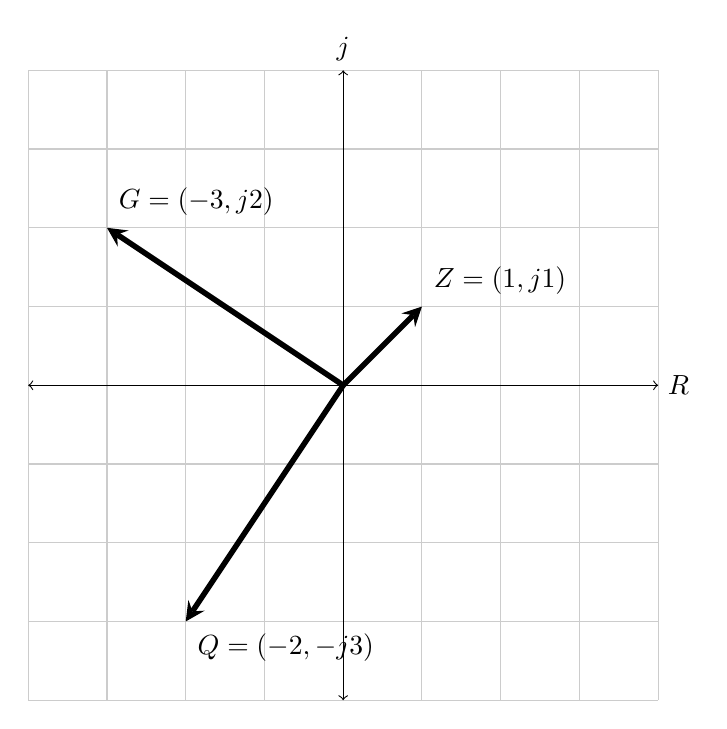
\begin{tikzpicture}
        \draw[thin,gray!40] (-4,-4) grid (4,4);
        \draw[<->] (-4,0)--(4,0) node[right] {$R$};
        \draw[<->] (0,-4)--(0,4) node[above]{$j$};
        \draw[line width=2pt,black,-stealth](0,0)--(1,1) node[anchor=south west]{${Z=(1,j1)}$};
        \draw[line width=2pt,black,-stealth](0,0)--(-3,2) node[anchor=south west]{${G=(-3,j2)}$};
        \draw[line width=2pt,black,-stealth](0,0)--(-2,-3) node[anchor=north west]{${Q=(-2,-j3)}$};
    \end{tikzpicture}
    \caption{Ejemplo de representacion de numero en el plano complejo}
    \label{fig:EjmNc}
\end{figure}
Como se puede intuir en al figura\ref{fig:EjmNc} acada punto del plano complejo le corresponde un valor imaginario y uno complejo, formando un espacio vectorial. También se pude apreciar que ambas unidades forman una base ortonormal.

Al ser el numero complejo un vector se puede escribir de distintas formas. La forma mas familiar de representar un numero complejo, para este punto sera de la forma cartesiana. Comparando un numero en el plano complejo y un vector en el plano de 2 dimensiones reales se puede apreciar la similitud.

\begin{figure}[H]%
\centering
    \begin{minipage}{0.5\textwidth}
    \centering
        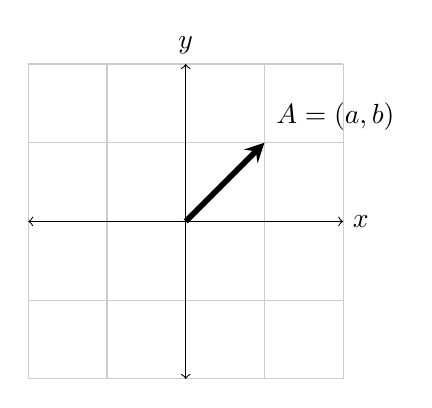
\begin{tikzpicture}
    \draw[thin,gray!40] (-2,-2) grid (2,2);
    \draw[<->] (-2,0)--(2,0) node[right] {$x$};
    \draw[<->] (0,-2)--(0,2) node[above]{$y$};
    \draw[line width=2pt,black,-stealth](0,0)--(1,1) node[anchor=south west]{${A=(a,b)}$};
\end{tikzpicture}
\caption*{$A=\hat{x}\cdot a+\hat{y}\cdot b$}
    \end{minipage}%
    \begin{minipage}{0.4\textwidth}
    \centering
        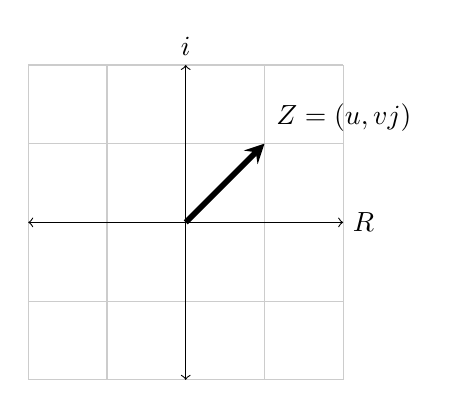
\begin{tikzpicture}
        \draw[thin,gray!40] (-2,-2) grid (2,2);
        \draw[<->] (-2,0)--(2,0) node[right] {$R$};
        \draw[<->] (0,-2)--(0,2) node[above]{$i$};
        \draw[line width=2pt,black,-stealth](0,0)--(1,1) node[anchor=south west]{${Z=(u,vj)}$};
\end{tikzpicture}
\caption*{$Z=u+j\cdot v$}
    \label{fig:test2}
    \end{minipage}%
    \caption{Comparación entre un numero complejo y un vector de 2 dimensiones reales}
    \label{fig:compri}
\end{figure}
En la figura:\ref{fig:compri} se muestra un vector real de 2 dimensiones $A$, compuesto por 2 componentes $a$ y $b$ ambos componentes están multiplicando a un versor de la base ($\hat{x}\ ,\ \hat{y}$). De manera similar también se muestra un numero complejo $Z$ el cual esta conformado por $u$ y $v$, $\ u$ siendo la parte real y $\ v$ siendo la parte imaginaria, ya que $\ v$ esta multiplicando la unidad imaginaria.
Las otras representaciones de un numero complejo son la forma polar y la forma exponencial.
\unsubsection{Forma polar}
La forma polar de un numero complejo tiene por datos el ángulo con respecto a el eje real (por convención), comúnmente llamado argumento y el modulo del numero complejo. Plateando un numero complejo de la forma:
\begin{equation}\label{eq:polz}
    z=x+jy
\end{equation}
\begin{figure}[H]
    \centering
        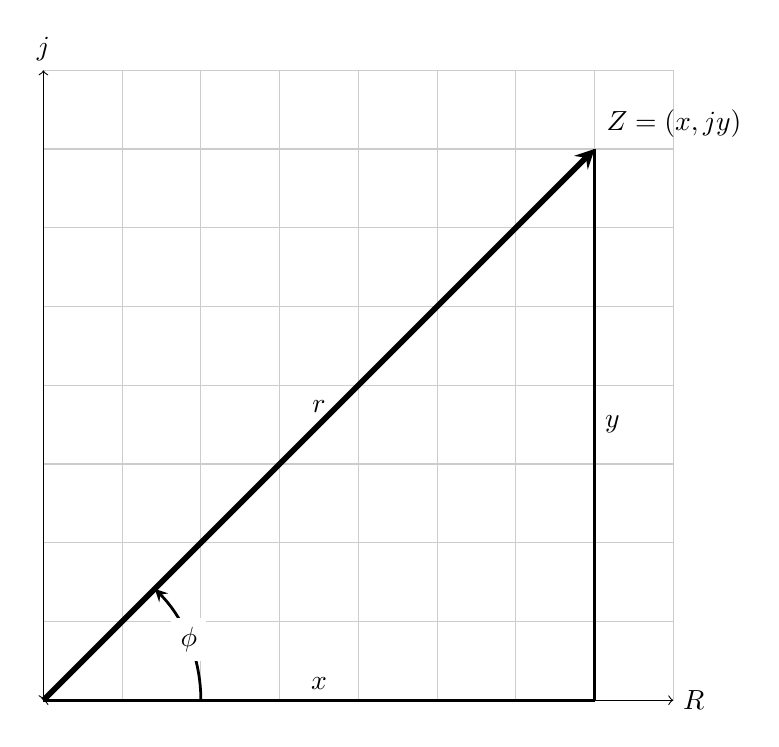
\begin{tikzpicture}
        \draw[thin,gray!40] (0,0) grid (8,8);
        \draw[<->] (0,0)--(8,0) node[right] {$R$};
        \draw[<->] (0,0)--(0,8) node[above]{$j$};
        \draw[line width=2pt,black,-stealth](0,0)--node[above]{$r$}(7,7) node[anchor=south west]{${Z=(x,jy)}$};
        \draw[line width=1pt,black,-](7,0)-- node[right]{$y$} (7,7);
        \draw[line width=1pt,black,-](0,0)-- node[above]{$x$}(7,0);
        \draw[line width=1pt,black,-stealth] (2,0) arc (0:45:2) node [midway,fill=white]{$\phi$};
\end{tikzpicture}
\caption{Planteo para la definición de la forma polar}
    \label{fig:Polar}
\end{figure}
Tomando en cuenta lo mostrado en la figura\ref{fig:Polar} podemos deducir que el modulo de un numero complejo es
\begin{equation}\label{eq:polr}
    r=\sqrt{x^2+y^2}
\end{equation}
Y además:
\begin{equation}\label{eq:polt}
    \phi=\arctan{(\dfrac{y}{x})}
\end{equation}
Por lo tanto:
\begin{equation}\label{eq:polx}
    x=r\cdot\cos{(\phi)}
\end{equation}
\begin{equation}\label{eq:poly}
    y=r\cdot\sin{(\phi)}
\end{equation}
Y por ultimo remplazndo \ref{eq:polx} y \ref{eq:poly} en \ref{eq:polz} obtenemos la forma final de un numero complejo en su forma polar:
\begin{equation}\label{eq:defPol}
    z=x+yj \llrah \ z=r\cdot[\cos{(\phi)}+j\sen{(\phi)}]
\end{equation}
Esta ecuación nos deja al descubierto una propiedad muy interesante de los números complejos. Al estar la forma polar definida a partir de cosenos y senos nos da a entender que varios números complejo de mismo modulo y distinto argumento pueden ser iguales, ya que el seno y el coseno son funciones periódicas en $2\pi$. 
\begin{figure}[H]%
\centering
    \begin{minipage}{0.5\textwidth}
    \centering
        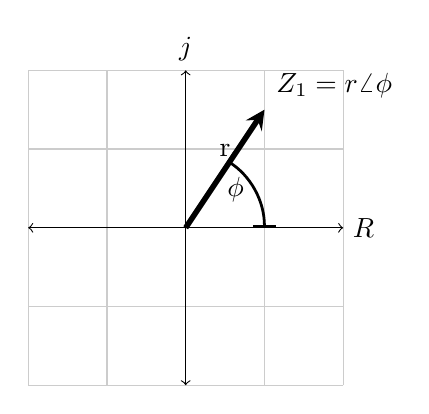
\begin{tikzpicture}
        \draw[thin,gray!40] (-2,-2) grid (2,2);
        \draw[<->] (-2,0)--(2,0) node[right] {$R$};
        \draw[<->] (0,-2)--(0,2) node[above]{$j$};
        \draw[line width=2pt,black,-stealth](0,0)--node[above]{r}(1,1.5) node[anchor=south west]{$Z_1=r\angle{\phi}$};
        \draw[line width=1pt,black,|-|] (1,0) arc (0:58:1) node [midway, left]{$\phi$};
    \end{tikzpicture}
    \end{minipage}%
    \begin{minipage}{0.4\textwidth}
    \centering
       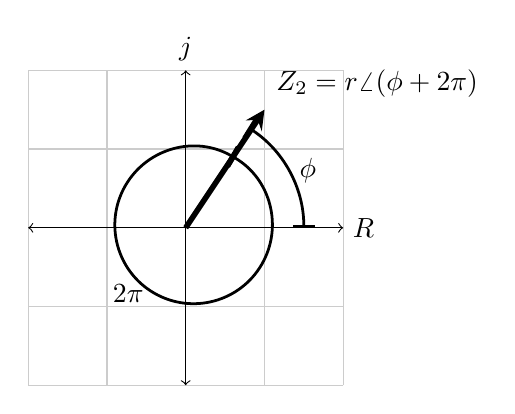
\begin{tikzpicture}
        \draw[thin,gray!40] (-2,-2) grid (2,2);
        \draw[<->] (-2,0)--(2,0) node[right] {$R$};
        \draw[<->] (0,-2)--(0,2) node[above]{$j$};
        \draw[line width=2pt,black,-stealth](0,0)--node[above]{}(1,1.5) node[anchor=south west]{$Z_2=r\angle{(\phi+2\pi)}$};
        \draw[line width=1pt,black,|-|] (0.6,0.902) arc (60:420:1) node [midway, left]{$2\pi$};
        \draw[line width=1pt,black,|-|] (1.5,0) arc (0:58:1.5) node [midway, right]{$\phi$};
    \end{tikzpicture}
    \label{fig:Perz}
    \end{minipage}%
    \caption{Comparación entre números complejos de igual modulo y argumentos $\phi_1$ y $\phi_2=2\pi+\phi_1$}
    \label{fig:Perio}
\end{figure}
\begin{figure}[H]
\centering
    \pgfplotsset{compat = newest}
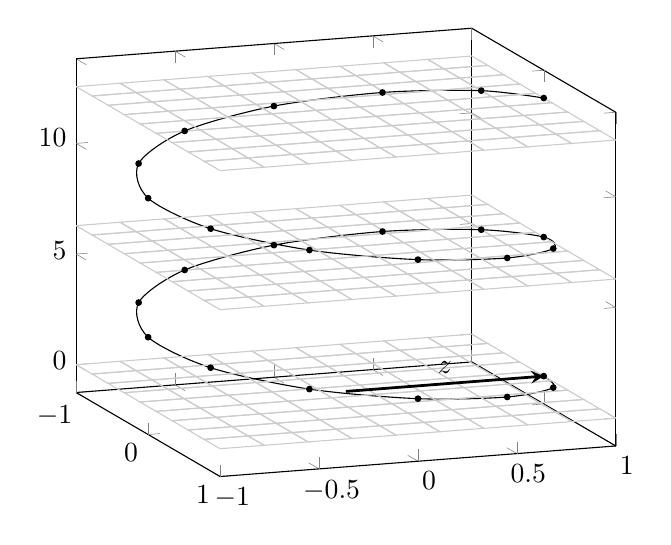
\begin{tikzpicture}
\begin{axis}[view={70}{15}]
    \addplot3+ [mark options={scale=0.5,fill=black,draw=black,},smooth,black,domain=0:4*pi,samples y=0] ({sin(deg(x))},{cos(deg(x))},{x});
    \addplot3+ [thin,no markers,mesh,draw=gray!40,domain=-1:1,samples=10] {2*pi};
    \addplot3+ [thin,no markers,mesh,draw=gray!40,domain=-1:1,samples=10] {0};
    \addplot3+ [thin,no markers,mesh,draw=gray!40,domain=-1:1,samples=10] {4*pi};
    \draw [line width=1pt,black,-stealth](0,0,0)--(0,1,0) node[midway, above]{$z$};
\end{axis}
\end{tikzpicture}
\caption{Representación de un numero $z=1[\cos{(\phi)}+j\sen{(\phi)}]$ siendo $\phi$ una variable correspondiente al eje $z$.}

    \label{fig:PerioC3}
\end{figure}
En la figura \ref{fig:PerioC3} se muestra un numero complejo al que se le modifica el argumento expresado en eje $z$, modificando sus coordenadas $(x,jy)$. Cuando el eje $z=2\pi$ se puede apreciar como el numero complejo toma las mismas coordenadas $(x,jy)$ que cuando $z=0$, lo mismo cuando $z=4\pi$.  
Por esta razón se debe restringir los valores que puede tomar el argumento en un intervalo de modulo $2\pi$, ya que otros argumentos que se salgan fuera de el intervalo definido pueden ser representados dentro del mismo intervalo. Nos quedaremos con la notación recomendada por la cátedra, la cual indica que el argumento esta restringido en $-\pi<\phi\leq\pi$
\begin{figure}[H]
    \centering
        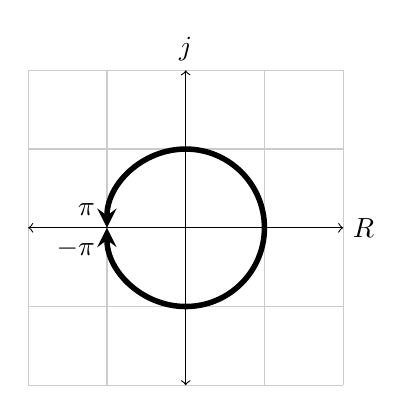
\begin{tikzpicture}
        \draw[thin,gray!40] (-2,-2) grid (2,2);
        \draw[<->] (-2,0)--(2,0) node[right] {$R$};
        \draw[<->] (0,-2)--(0,2) node[above]{$j$};
        \draw[line width=2pt,black,-stealth] (1,0) arc (0:180:1) node [anchor=south east]{$\pi$};
        \draw[line width=2pt,black,-stealth] (1,0) arc (0:-180:1) node [anchor=north east]{$-\pi$};
    \end{tikzpicture}
    \caption{Intervalo del argumento}
    \label{fig:interphi}
\end{figure}
\unsubsection{Forma exponencial}
Ser capaces de representar un numero complejo en su forma exponencial va a probar ser una de las herramientas más útiles de la materia. Para poder expresar un numero complejo en su forma exponencial se debe presentar las identidades trigonométricas definidas por las identidades de Euler, las cuales solo van a ser presentadas y no demostradas.
Las identidades trigonométricas son:
\begin{equation}\label{eq:eulers}
    \sin{(x)}=\cfrac{1}{2j}\cdot(e^{j\phi}-e^{-j\phi})
\end{equation}
\begin{equation}\label{eq:eulerc}
    \cos{(x)}=\cfrac{1}{2}\cdot(e^{j\phi}+e^{-j\phi})
\end{equation}
Remplazando \ref{eq:eulers} y \ref{eq:eulerc} en la ecuación de la defunción de la forma polar \ref{eq:defPol} obtenemos:
\begin{equation}
\begin{aligned}
      z=r\cdot[\cos{(\phi)}+j\sen{(\phi)}] \quad\Longrightarrow\quad z&=r\cdot[(\cfrac{1}{2}\cdot(e^{j\phi}+e^{-j\phi})+\cfrac{\bcancel{j}}{2\bcancel{j}}\cdot(e^{j\phi}-e^{-j\phi})]\\
      &=r[\cfrac{1}{2}\cdot(e^{j\phi}+e^{j\phi}+\bcancel{e^{-j\phi}}-\bcancel{e^{-j\phi}}]\\
      &=r[\bcancel{\cfrac{1}{2}}\cdot \bcancel{2}e^{j\phi}]\\
\end{aligned}
\end{equation}
\begin{equation}\label{eq:defExp}
    z=re^{j\phi}
\end{equation}
De esta manera obtenemos la definición de la forma exponencial. Esta manera de explicarlo es un poco ambigua ya que deja muchas preguntas sin contestar, cada uno elige hasta donde seguir el conejo blanco.
\unsection{Operaciones básicas y propiedades}
\unsubsection{Suma} 
    El plano complejo sigue las normas de un espacio vectorial por lo tanto la suma se computa componente a componente, en nuestro caso al ser un espacio vectorial de 2 dimensiones la suma se define como:
        \begin{equation}\label{eq:sum}
          z_1+z_2 \Rightarrow (x_1\ ,\ jy_1)+(x_2\ ,\ jy_2)=(x_1+x_2\ ,\ jy_1+jy_2))\\
        \end{equation}
    \begin{figure}[H]
        \centering
        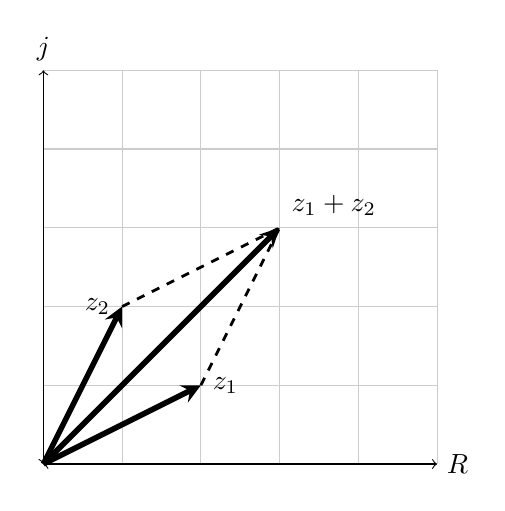
\begin{tikzpicture}
        \draw[thin,gray!40] (0,0) grid (5,5);
        \draw[<->] (0,0)--(5,0) node[right] {$R$};
        \draw[<->] (0,0)--(0,5) node[above]{$j$};
       \draw[line width=2pt,black,-stealth](0,0)--(1,2) node[left]{${z_2}$};
       \draw[line width=2pt,black,-stealth](0,0)--(2,1) node[right]{${z_1}$};
       \draw[line width=2pt,black,-stealth](0,0)--(3,3) node[anchor=south west]{${z_1+z_2}$};
       \draw[line width=1pt,black,dashed](1,2)--(3,3);
       \draw[line width=1pt,black,dashed](2,1)--(3,3);
    \end{tikzpicture}
    \caption{Representacion de la suma entre 2 numeros complejos}
        \label{fig:sumaC}
    \end{figure}
    Intuitivamente podemos apreciar que el elemento neutro de la suma es el vector $(0,0)$, por lo tanto el 0 en el plano complejo es el vector nulo.
        \begin{equation}\label{eq:sumnul}
            (x_1\ ,\ jy_1)+(0\ ,\ j0) \lrah (x_1+0\ ,\ jy_1+j0)=x_1+jy_1 \Rightarrow z_1+0 \\
        \end{equation}
    La suma hereda todas las propiedades de la suma en un espacio vectorial de $n$ dimensiones reales.
    \begin{itemize}
        \item Conmutatividad:
        \begin{equation}
            (a\ ,\ jb)+(\hat{a}\ ,\ j\hat{b})=(\hat{a}\ ,\ j\hat{b})+(a\ ,\ jb)
        \end{equation}
        \item Asociatividad:
        \begin{equation}
            [(a\ ,\ jb)+(\hat{a}\ ,\ j\hat{b})]+(\bar{a}\ ,\ j\bar{b})=(a\ ,\ jb)+[(\hat{a}\ ,\ j\hat{b})+(\bar{a}\ ,\ j\bar{b})]
        \end{equation}
        \item Elemento neutro:
        \begin{equation}
             (a\ ,\ jb)+(0\ ,\ j0) \lrah (a+0\ ,\ jb+j0)=a+jb 
        \end{equation}
        \item Opuesto (necesario para la resta):
        \begin{equation}
            -(a\ ,\ jb)=(-a\ ,\ -jb)
        \end{equation}
        Si sumamos a un $z$ su opuesto nos da como resultado el elemento neutro de la suma:
         \begin{equation}
            z-z=(a\ ,\ jb)-(a\ ,\ jb)\lrah \bcancel{(a-a)}+j\bcancel{(b-b)} = 0+j0
        \end{equation}
        Si restamos un $z_0=(x_0+jy_0)$ a un $z_1=(x_1+jy_1)$ obtendremos la expresión:
        \begin{equation}
            z_1-z_0=(x_1+jy_1)-(x_0+jy_0) \lrah z_0-z_1=(x_1-x_0)+j(y_1-y_0)
        \end{equation}
        \begin{figure}[H]
            \centering
            \begin{minipage}{0.4\textwidth}
            \centering
                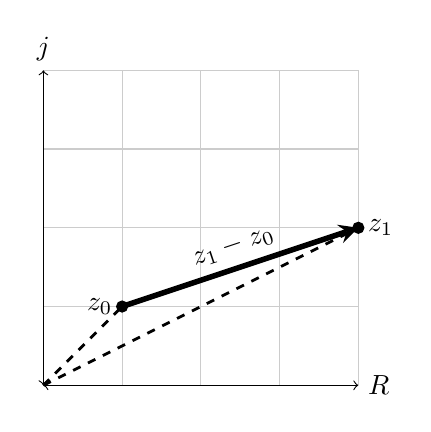
\begin{tikzpicture}
    \draw [thin,gray!40] (0,0) grid (4,4);
    \draw[<->] (0,0)--(4,0) node[right] {$R$};
    \draw[<->] (0,0)--(0,4) node[above]{$j$};
    \coordinate (a) at (1,1);
    \coordinate (b) at (4,2);
    \draw[fill=black] (a) circle(2pt) node[left]{$z_0$};
    \draw[fill=black] (b) circle(2pt) node[right]{$z_1$};
    \draw[line width=2pt,black,-stealth] (a)--(b) node[midway, above, sloped]{$z_1-z_0$};
    \draw[line width=1pt,black,dashed] (0,0)--(a);
    \draw[line width=1pt,black,dashed] (0,0)--(b);
\end{tikzpicture}
            \end{minipage}%
            \begin{minipage}{0.4\textwidth}
            \centering
                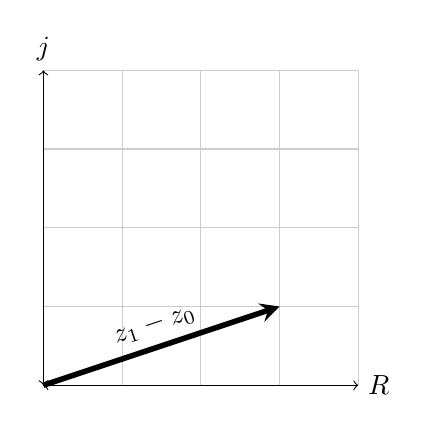
\begin{tikzpicture}
    \draw [thin,gray!40] (0,0) grid (4,4);
    \draw[<->] (0,0)--(4,0) node[right] {$R$};
    \draw[<->] (0,0)--(0,4) node[above]{$j$};
    \draw[line width=2pt,black,-stealth] (0,0)--(3,1) node[midway, above, sloped]{$z_1-z_0$};
\end{tikzpicture}

            \end{minipage}
            \caption{Resta de números complejos}
            \label{fig:RestC}
        \end{figure}
        Entonces restar 2 numero complejos da como resultado un vector de origen en $z_0$ y punto final $z_1$ y también se pude representar como un vector con origen en el punto $(0,j0)$ y final $(x_0-x_1)+j(y_0-y_1)$
    \end{itemize}
\unsubsection{Multiplicación} 
    La multiplicación, al ser el plano complejo un campo vectorial, se computa multiplicando todos los elementos entre ellos y recordando que $j\cdot j=-1$ de la ecuación \ref{eq:jj}. Entonces: 
        \begin{equation}\label{eq:mul}
        \begin{aligned}
            z_1\cdot z_2 \Rightarrow (x_1+y_1j)\cdot(x_2+y_2j)&=(x_1\cdot x_2)+(x_1\cdot y_2j)+(x_2\cdot y_1j)+(y_1j\cdot y_2j)\\
             &=(x_1\cdot x_2)+j^2(y_1\cdot y_2)+j(x_1\cdot y_2+x_2\cdot y_1)\\
             &=(x_1\cdot x_2-y_1\cdot y_2)+j(x_1\cdot y_2+x_2\cdot y_1)
        \end{aligned}
        \end{equation}
    La multiplicación en la forma exponencial es mucho mas simple, recordando la propiedad de la potencia $a^b \cdot a^c=a^{(b+c)}$:
    \begin{equation}\label{eq:mulE}
        z_1\cdot z_2 = r_1e^{j\theta}\cdot r_2e^{j\phi} \lrah z_1\cdot z_2 = (r_1 r_2)e^{j(\theta+\phi)}
    \end{equation}
    Por lo tanto la multiplicación de 2 números complejos da como resultados otro numero complejo, el cual su modulo es la multiplicación de los 2 primeros módulos y su argumento es la suma de los argumentos de los factores. Con este concepto es trivial desarrollar la multiplicación en forma polar, ya que tenemos todos los datos necesrios.
    \begin{equation*}
         z_1\cdot z_2=r_1[\cos{\theta}+j\sin{\theta}]\cdot r_2[\cos{\phi}+j\sin{\phi}]
    \end{equation*}
    \begin{equation}
        z_1\cdot z_2 =(r_1\cdot r_2)[\cos{(\theta +\phi)}+j \sin{(\theta +\phi})]
    \end{equation}
    De aquí se puede intuir que el elemento neutro de la multiplicación es aquel numero complejo que tenga modulo igual a $1$ y argumento igual a $0$:
    \begin{equation}
        z_1\cdot z_n = r_1e^{j\theta}\cdot 1e^{j0} \Longrightarrow z_1\cdot z_n = (r_1 1)e^{j(\theta+0)}
    \end{equation}
    A través de la ecuación \ref{eq:defPol} podemos encontrar que:
    \begin{equation}
        z_n = 1\cdot[\cos{(0)}+j\sen{(0)}] = (1\ ,\ j0)
    \end{equation}
    Por lo tanto el elemento neutro de la multiplicación es el versor $(1\ ,\ j0)$, que es la unidad real.
    
    Un caso que cabe resaltar es la multiplicación por la unidad imaginaria $j$. Como se puede demostrar, la unidad imaginaria tiene un modulo igual a $1$ y argumento igual a $90^{\circ}$ o lo que viene siendo lo mismo $\pi/2$ radianes:
    \begin{equation}
        z_1\cdot j = r_1e^{j\theta}\cdot 1e^{j\frac{\pi}{2}} \Longrightarrow z_1\cdot j = (r_1 1)e^{j(\theta+\frac{\pi}{2})}
    \end{equation}
    o en cartesianas
    \begin{equation}
        z_1\cdot j = (a\ , \ jb)\cdot j \Longrightarrow (a\cdot j\ ,\ j\cdot jb)=(-b\ ,\ ja)
    \end{equation}
   Como se pude apreciar, multiplicar cualquier numero complejo por $j$ da como resultado el mismo vector rotado $90^{\circ}$
   \begin{figure}[H]
       \centering
       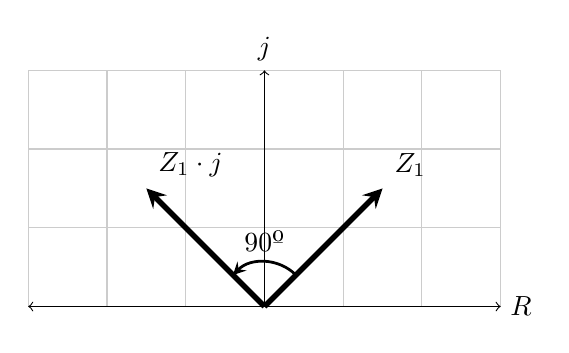
\begin{tikzpicture}
        \draw[thin,gray!40] (-3,0) grid (3,3);
        \draw[<->] (-3,0)--(3,0) node[right] {$R$};
        \draw[<->] (0,0)--(0,3) node[above]{$j$};
        \draw[line width=2pt,black,-stealth](0,0)--(1.5,1.5) node[anchor=south west]{$Z_1$};
        \draw[line width=2pt,black,-stealth](0,0)--(-1.5,1.5) node[anchor=south west]{$Z_1\cdot j$};
        \draw[line width=1pt,black,-stealth] (0.4,0.4) arc (45:135:0.566) node[midway, above]{90º};
\end{tikzpicture}
\caption{Numero complejo multiplicado por la unidad imaginaria}
       \label{fig:MultiC}
   \end{figure}
    Otro caso interesante en el análisis es el caso de multiplicar a un $z_1=(a\ ,\ jb)$ por $z_2=(a\ ,\ -jb)$:
    \begin{equation}
    \begin{aligned}
        z_1\cdot z_2 \Rightarrow (a+jb)\cdot(a-jb)&=(a\cdot a)+(a\cdot jb)+(a\cdot -jb)+(jb\cdot -jb)\\
             &=a^2+j^2(b\cdot -b)+j(a\cdot b-a\cdot b)\\
             &=a^2+b^2
    \end{aligned}
    \end{equation}
    El resultado de esta multiplicación nos da un numero completamente real, que es igual al cuadrado del modulo de $z$. Por esta propiedad a $z_2$ se le suele llamar el conjugado de $z_1$. El conjugado ($z^*$) de un numero complejo es, entonces, otro numero complejo con igual parte real y opuesta parte imaginaria, esto se puede pensar como una reflexión con respecto al eje real.
    \begin{figure}[H]
        \centering
        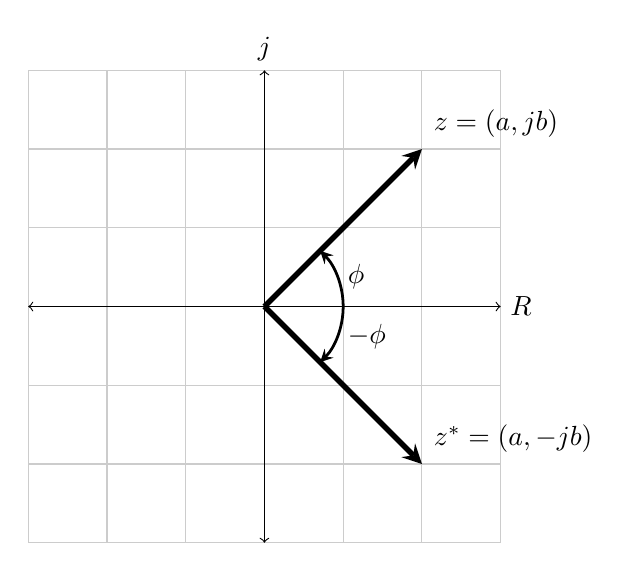
\begin{tikzpicture}
        \draw[thin,gray!40] (-3,-3) grid (3,3);
        \draw[<->] (-3,0)--(3,0) node[right] {$R$};
        \draw[<->] (0,-3)--(0,3) node[above]{$j$};
       \draw[line width=2pt,black,-stealth](0,0)--(2,2) node[anchor=south west]{${z=(a,jb)}$};
       \draw[line width=2pt,black,-stealth](0,0)--(2,-2) node[anchor=south west]{${z^*=(a,-jb)}$};
       \draw[line width=1pt,black,-stealth] (1,0) arc (0:45:1) node [midway, right]{$\phi$};
        \draw[line width=1pt,black,-stealth] (1,0) arc (0:-45:1) node [midway, right]{$-\phi$};
    \end{tikzpicture}
    \caption{conjugado de un numero complejo}
        \label{fig:ConjC}
    \end{figure}
    Como se deja intuir en la figura \ref{fig:ConjC}, en su forma exponencial o polar, el conjugado de $z$ es otro numero complejo de igual modulo y argumento opuesto.
    \begin{equation}
       z= re^{j\phi} \lrah z^*= re^{-j\phi}
    \end{equation}
    Enumerando las propiedades de la multiplicación 
\begin{itemize}
    \item Conmutatividad:
        \begin{equation}
            (a\ ,\ jb)\cdot(\hat{a}\ ,\ j\hat{b})=(\hat{a}\ ,\ j\hat{b})\cdot(a\ ,\ jb)
        \end{equation}
    \item Asociatividad:
        \begin{equation}
            [(a\ ,\ jb)\cdot(\hat{a}\ ,\ j\hat{b})]\cdot(\bar{a}\ ,\ j\bar{b})=(a\ ,\ jb)\cdot[(\hat{a}\ ,\ j\hat{b})\cdot(\bar{a}\ ,\ j\bar{b})]
        \end{equation}
    \item Distributiva:
    \begin{equation}
        (a\ ,\ jb)\cdot((\hat{a}\ ,\ j\hat{b})+\lambda)=  (a\ ,\ jb)\cdot(\hat{a}\ ,\ j\hat{b})+\lambda \cdot (a\ ,\ jb)
    \end{equation}
    \item Elemento neutro:
        \begin{equation}
             (a\ ,\ jb)\cdot(1\ ,\ j0) \lrah (a\cdot 1 + \bcancel{a\cdot j0}) +\ (jb\cdot 1+\bcancel{jb\cdot j0}))=a+jb 
        \end{equation}
    \item Inverso: 
    En esta propiedad nos vamos a detener ya que no es trivial el análisis.
    La inversa de la multiplicación es la división, que es $z_1/z_2$ también se pude escribir como $z_1\cdot z_2^{-1}$ nos faltaría definir como se computa el inverso de un numero complejo:
    \begin{equation*}
        \cfrac{1}{z}=\cfrac{1}{a+jb} \lrah \cfrac{1}{a+jb}\cdot\cfrac{a-jb}{a-jb}=\cfrac{a-jb}{a^2+b^2}
    \end{equation*}
    \begin{equation}
        \cfrac{1}{z}=\cfrac{a}{a^2+b^2}-j\cfrac{b}{a^2+b^2}
    \end{equation}
    Es necesario recalcar que se multiplica $1/z$ por $z^*/z^*$ para eliminar la parte imaginaria del denominador.
    
    Se pude probar lo mismo de manera mas sencilla representando a $z$ en su forma exponencial y recordando la propiedad$1/a^x=a^{-x}$:
    \begin{equation}
        \cfrac{1}{z}=\cfrac{1}{re^{j\theta}} \lrah \cfrac{1}{z}=\cfrac{1}{r}e^{-j\theta}
    \end{equation}
    Entonces el inverso de un numero complejo da como resultado otro numero complejo de modulo $1/r$ y argumento $-\theta$.
    Con esto explicado podemos razonar que  dividir un $z_1$ por un $z_2$ no es mas que multiplicar $z_1$ por el inverso de $z_2$:
    \begin{equation}
        \cfrac{z_1}{z_2}= r_1e^{j\theta}\cdot \cfrac{1}{r_2}e^{-j\phi} \lrah 
        \begin{cases}
            \cfrac{z_1}{z_2} = (\cfrac{r_1}{r_2})e^{j(\theta-\phi)}\\
            \\
            \cfrac{z_1}{z_2} =(\cfrac{r_1}{r_2})[\cos{(\theta -\phi)}+j \sin{(\theta -\phi})] 
        \end{cases}
    \end{equation}
    
    Si multiplicamos a un $z$ por $1/z$ obtendremos el elemento neutro de la multiplicación:
     \begin{equation}
        z\cdot \cfrac{1}{z}=re^{(j\theta)}\cfrac{1}{re^{j\theta}} \lrah \cfrac{z}{z}=\bcancel{\cfrac{r}{r}}e^{\bcancel{j\theta-j\theta}} = 1e^{j0} = (1,j0)
    \end{equation}
    
    \end{itemize}
\unsubsection{Potenciación} 
    La potenciación de un numero $z$ en $n$ no es mas que la multiplicación sucesiva de $z$ $n$ veces. Se recomienda computar la potenciación en la forma polar o exponencial:
    \begin{equation}\label{eq:defPot}
        z^n=\begin{cases}
        (re^{j\theta})^n \lrah z^n =r^ne^{j\theta \cdot n} \\
        \\
        (r[\cos{(\theta)}+j\sin{(\theta)}])^n \lrah z^n = (r^n)[\cos{(\theta \cdot n)}+j \sin{(\theta \cdot n})]
        \end{cases}
    \end{equation}
    En términos de propiedades es distributiva en la multiplicación:
    \begin{equation}
        ((a\ ,\ jb)\cdot \lambda)^n = (a\ ,\ jb)^n\cdot \lambda^n
    \end{equation}
    Y elevar cualquier numero imaginario por $0$ da como resultado la unidad real, partiendo de \ref{eq:defPot}:
    \begin{equation}
        z^0=(r^0)[\cos{(\theta \cdot 0)}+j \bcancel{\sin{(\theta \cdot 0}})] = 1\cdot[1+j0] = (1\ ,\ j0)
    \end{equation}
\unsubsection{Radicación}
    La radicación es un poco mas compleja que la potenciación, se recomienda ver la unidad de funciones complejas y mapeo antes de ver este tema.
    Se debe recordar que los números complejos son periódicos en $2\pi$ por lo tanto y haciendo uso de la ecuación \ref{eq:defPol} se puede escribir un numero complejo de la siguiente manera:
    \begin{equation}
        z = r[\cos{(\theta + 2\pi k)}+j\sin{(\theta + 2\pi k)}] \llrah \ z = re^{j(\theta+2\pi k)}
    \end{equation}
    $k$ siendo cualquier numero entero.
    Esto es necesario ya que la raíz tiene múltiples respuestas a un mismo numero complejo ya que afecta el carácter periódico de la misma. Recordando que la raíz enésima se puede expresar como $\sqrt[n]{a}=a^{1/n}$ y la definición de la potenciación \ref{eq:defPot}:
    \begin{equation}\label{eq:defRad}
        z^{\frac{1}{n}} = (re^{j(\theta+2\pi k)})^{\frac{1}{n}}
        \begin{cases}
             z^{\frac{1}{n}} = r^{\frac{1}{n}}e^{j(\frac{\theta+2\pi k}{n})}\\
             \\
             z^{\frac{1}{n}} = r^{\frac{1}{n}}[\cos{(\frac{\theta + 2\pi k}{n})}+j\sin{(\frac{\theta + 2\pi k}{n})}]
        \end{cases}
    \end{equation}
    Como se pude apreciar la radicación de un numero complejo da otro numero complejo de modulo $r^{(1/n)}$, pero lo interesante pasa por ver que le sucede al argumento.
    Ahora el argumento esta dado por la expresión $\frac{\theta + 2\pi k}{n}$ que la podemos descomponer en dos partes, $\frac{\theta}{n}$ y $\frac{2\pi k}{n}$, recordemos que $n$ es una constante y $k$ una variable que solo puede tomar valores de números enteros. La segunda expresión le da el carácter periódico al numero complejo pero esta expresión dejo de ser igual a un múltiplo de $2\pi$, para que este vuelva a ser el caso $k$ debe ser igual a $\lambda \cdot n$, $\lambda$ siendo un numero entero.
    \begin{equation*}
        \cfrac{2\pi k}{n}
        \begin{cases}
            k=\lambda n \lrah \cfrac{2\pi k}{n} =  2\pi \lambda \\
            \\
            k \neq \lambda \lrah \cfrac{2\pi k}{n}
        \end{cases}
    \end{equation*}
    Por lo tanto existen $n$ distintos argumentos que no se repiten en $2\pi$.
    
    Tomando en cuenta esto existen $n$ respuestas a la raíz enésima de un numero complejo:
    \begin{equation}
    \begin{aligned}
         z^{\frac{1}{n}}= & r^{\frac{1}{n}}[\cos{(\frac{\theta + 2\pi \cdot 0}{n})}+j\sin{(\frac{\theta + 2\pi \cdot 0}{n})}]\\
                        & r^{\frac{1}{n}}[\cos{(\frac{\theta}{n} +\frac{2\pi \cdot 1}{n})}+j\sin{(\frac{\theta}{n} +\frac{2\pi \cdot 1}{n})}]\\
                        & r^{\frac{1}{n}}[\cos{(\frac{\theta}{n} +\frac{2\pi \cdot 2}{n})}+j\sin{(\frac{\theta}{n} +\frac{2\pi \cdot 2}{n})}]\\
                        & r^{\frac{1}{n}}[\cos{(\frac{\theta}{n} +\frac{2\pi \cdot 3}{n})}+j\sin{(\frac{\theta}{n} +\frac{2\pi \cdot 3}{n})}]\\
                        &\hspace{3.6cm} \cdot \\
                        &\hspace{3.6cm} \cdot \\
                        &\hspace{3.6cm} \cdot \\
                        &\hspace{3.37cm} \ldots \\
                        & r^{\frac{1}{n}}[\cos{(\frac{\theta}{n} +\frac{2\pi \cdot (n-2)}{n})}+j\sin{(\frac{\theta}{n} +\frac{2\pi \cdot (n-2)}{n})}]\\
                        & r^{\frac{1}{n}}[\cos{(\frac{\theta}{n} +\frac{2\pi \cdot (n-1)}{n})}+j\sin{(\frac{\theta}{n} +\frac{2\pi \cdot (n-1)}{n})}]\\
    \end{aligned}
    \end{equation}
    Planteando el ejemplo de numero complejo $(\-0.5735,\ j0.819)$:
    \begin{enumerate}
        \item Obtenemos la expresión en la forma polar, para este caso este numero tiene un modulo de $1$ y un argumento de $125^{\circ}$ que equivalen a $\frac{25}{36}\pi$ radianes:
        \begin{equation}
         z= 1e^{j\pi(\frac{25}{36}+2k)} \llrah z = 1[\cos{(125^{\circ} + 360^{\circ} k)}+j\sin{(125^{\circ} + 360^{\circ} k)}]
        \end{equation}
        \item Planteamos una radicación de orden 5 por ejemplo, recordando la definición de radicación \ref{eq:defRad}:
        \begin{equation}
            \sqrt[5]{z}=\sqrt[5]{1} \cdot [\cos{\frac{(125^{\circ} + 360^{\circ} k)}{5}}+j\sin{\frac{(125^{\circ} + 360^{\circ}}{5} k)}]
        \end{equation}
        \begin{equation}\label{eq:RadCej} 
            \sqrt[5]{z}=1[\cos{(25^{\circ} + 72^{\circ} k)}+j\sin{(25^{\circ} + 72^{\circ}k)}]
        \end{equation}
        Podemos ver que el argumento de las raices van a variar en $72^{\circ}$ uno del otro y que solo nos hace falta valuar $0\leqslant k \leqslant 4$ ya que cunado $k=5$ lo que suma a los $25^{\circ}$ va a ser igual a $360^{\circ}$ o 
 $2\pi$ radianes y se van a empezar a repetir los argumentos.
    \end{enumerate}
\begin{figure}[H]
    \centering
    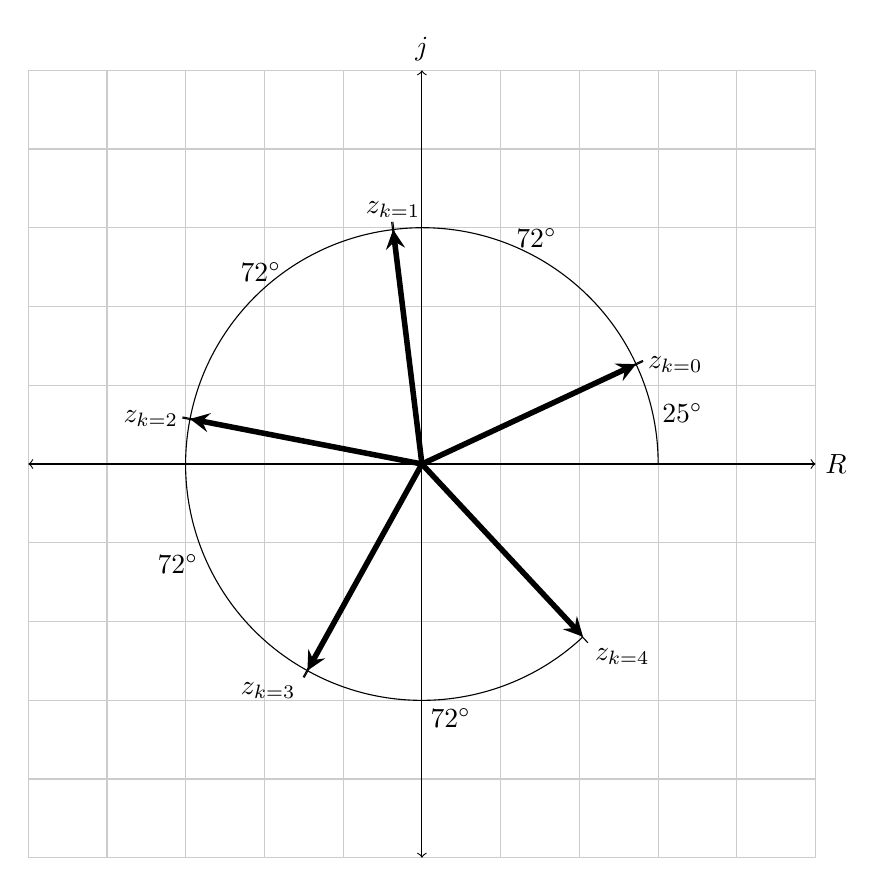
\begin{tikzpicture}
        \draw[thin,gray!40] (-5,-5) grid (5,5);
        \draw[<->] (-5,0)--(5,0) node[right] {$R$};
        \draw[<->] (0,-5)--(0,5) node[above]{$j$};
        \draw[line width=2pt,black,-stealth](0,0)--(2.72,1.268) node[right]{${z_{k=0}}$};
        \draw[line width=2pt,black,-stealth](0,0)--(-0.3656,2.977) node[above]{${z_{k=1}}$};
        \draw[line width=2pt,black,-stealth](0,0)--(-2.945,0.5724) node[left]{${z_{k=2}}$};
        \draw[line width=2pt,black,-stealth](0,0)--(-1.4544,-2.624) node[anchor=north east]{${z_{k=3}}$};
        \draw[line width=2pt,black,-stealth](0,0)--(2.046,-2.194) node[anchor=north west]{${z_{k=4}}$};
        \draw[|-|] (3,0) arc (0:25:3) node [midway, right]{$25^{\circ}$};
        \draw[|-|] (2.72,1.268) arc (25:97:3) node [midway,above]{$72^{\circ}$};
        \draw[|-|] (-0.3656,2.977) arc (97:169:3) node [midway, above]{$72^{\circ}$};
        \draw[|-|] (-2.945,0.5724) arc (169:241:3) node [midway, left]{$72^{\circ}$};
        \draw[|-|] (-1.4544,-2.624) arc (241:313:3) node [midway, below]{$72^{\circ}$};
    \end{tikzpicture}
    \caption{Representación de la ecuación \ref{eq:RadCej} en el intervalo marcado}
    \label{fig:RadC}
\end{figure}
\unsubsection{Logaritmo natural}
El logaritmo natural de un numero complejo es la inversa de la forma exponencial. La única forma de computar el logaritmo natural cómodamente es con la forma exponencial del numero. Recordando la propiedades de los logaritmos $\ln{(e)}=1$, $\ln{(a\cdot b)}=\ln{(a)}+\ln{(b)}$ y $\ln{(a^b)}=b\cdot \ln{(a)}$:
\begin{equation} \label{eq:defLnC}
    \ln{z}=\ln{(re^{j\theta})}\lrah \ln{z}=\ln{(r)}+j\theta
\end{equation}
Como vemos en la ecuación \ref{eq:defLnC} el logaritmo natural de un numero complejo, en su forma exponencial, da como resultado un otro numero complejo en forma cartesiana de parte real igual al logaritmo natural del radio y parte imaginaria igual a su argumento.
\unsection{Otros operadores}
Para los números complejos existen otras operaciones exclusivas que son útiles en el analisis complejo.
\begin{itemize}
    \item Operador $\Real{}$:
    Este operador devuelve la parte real de un numero complejo y descarta la parte imaginaria.
    \begin{equation}\label{eq:DefImagC}
        z=(a+jb) \lrah \Real{z}=a
    \end{equation}
     \item Operador $\Imag{}$: 
     Similar al operador $\Real{}$, este operador toma la parte imaginaria de un numero complejo y descarta la parte real
     \begin{equation}\label{eq:DefRealC}
         z=(a+jb) \lrah \Imag{z}=b
     \end{equation}
     \item Operador $*$:
      Aunque ya hayamos presentado el concepto de números conjugados, formalmente $*$ es un operador que devuelve el conjugado de un numero complejo.
      \begin{equation}\label{eq:DefConC}
          z=(a+jb) \lrah z^*=(a-jb)
      \end{equation}
      \item Operador modulo $||$:
      Este operador devuelve el modulo de un numero complejo:
      \begin{equation}\label{eq:DefModC}
          |z|=\sqrt{x^2+y^2} \llrah\ |z|=|re^{j\theta}|=r \llrah\ |z|=|r[\cos{\theta}+j\sin{\theta}]|=r
      \end{equation}
      Cuando el numero $z$ es escalado un $\lambda$ entonces el modulo estará multiplicado por $\lambda$:
      \begin{equation}
          |\lambda z|=\sqrt{(\lambda x)^2+(\lambda y)^2}\lrah\sqrt{\lambda^2(x^2+y^2)}=\lambda\sqrt{x^2+y^2}
      \end{equation}
      \begin{equation}
          |\lambda z|=\lambda|z|
      \end{equation}
      \item Operador $Arg$ o $\angle$:
      Este operador devuelve el argumento del modulo, siendo $z=x+jy$:
      \begin{equation}
          Arg(z)=\tan^{-1}{(\frac{y}{x})} \llrah\ Arg(re^{j\theta})=\angle\theta \llrah\ Arg(r[\cos{\theta}+j\sin{\theta}])=\angle\theta
      \end{equation}
      
     
\end{itemize}
%\chapter{Funciones complejas y mapeo}

\unsection{Introducción}
Una función compleja tiene dominio e imagen en 2 dimensiones ya que toma un numero complejo y lo transforma en otro numero complejo. Lo que quiere decir esto es que las funciones complejas tienen 2 variables independientes y 2 variables dependientes. Por esta cualidad para graficarlas correctamente necesitaríamos un sistema de representación en 4 dimensiones, 2 para las variables y otras 2 para las respuestas, lo cual es físicamente imposible. Otra forma de poder visualizar como se comportan las funciones complejas es graficar como se modifica el plano complejo a través de una función y otra forma es tomar elementos geométricos, como lineas y círculos y ver como son transformadas por la función. Llegar a poder visualizar como se comportan distintas funciones a través de este concepto es el objetivo de esta parte de la materia.

\unsection{Ecuación complejas}
Antes de saltar a funciones y mapeos deberíamos definir como funcionan las ecuaciones complejas. Una ecuación compleja se define de manera similar a una ecuación de una variable. La variable compleja se le sule denotar con una $z$. Una ecuación de ejemplo seria:
\begin{equation}\label{eq:ejmEQC}
    z^2+3=0
\end{equation}
Como en una ecuación de numero reales, el conjunto solución de la ecuación \ref{eq:ejmEQC} son todos aquellos números complejo que satisfagan la igualdad. En este caso es una ecuación de orden 2 así que vamos a obtener 2 respuestas. Los método de resolución aplicables son iguales al de una ecuación real, usando la formula de baskara por ejemplo o despejando $z$ para encontrar la condición que debe cumplir la variable. Partiendo de la ecuación \ref{eq:ejmEQC}:
\begin{equation}\label{eq:ejmEQCS1}
    \begin{aligned}
         z^2+3=0 \lrah z^2&=-3\\
                        \pm z&=\sqrt{-3}\\
                        z&=\pm \sqrt{-1\cdot 3}\\
                        z&=\pm \sqrt{-1}\cdot\sqrt{3}\\
                        z&=\pm j\sqrt{3}
    \end{aligned}
\end{equation}
A diferencia de las ecuaciones reales la incógnita $z$ es una incógnita de 2 dimensiones($z=x+jy$), por lo tanto una ecuación compleja puede subdividirse en la parte que restringe los valores reales y otra que rige los valores posibles de la parte imaginaria de $z$. Haciendo el planteo desde la ecuación \ref{eq:ejmEQC}:
\begin{equation}
    \begin{aligned}
     z^2+3=0 \lrah &(x+jy)^2+3=0\\
                      &(x+jy)\cdot(x+jy)=-3\\
                  &(x^2+(jy)^2)+(x\cdot jy + x\cdot jy)=-3
    \end{aligned}
\end{equation}
\begin{equation}
    (x^2-y^2)+j(2xy)=(-3\ ,\ j0)
\end{equation}
De aquí podemos separa la parte real de la respuesta con la parte real de la incógnita y lo mismo con las partes imaginarias, generando un sistema de ecuación.
\begin{equation}
(x^2-y^2)+j(2xy)=(-3\ ,\ j0)
    \begin{cases}
        x^2-y^2=-3\\
        2xy=0
    \end{cases}
\end{equation}
Resolviendo el sistema de ecuaciones llegaremos a la conclusión de que $x=0$ y $y=\pm \sqrt{3}$, recordando que $z=x+jy$ llegaremos a la misma solución que en la ecuación \ref{eq:ejmEQCS1}:
\begin{equation}
\begin{aligned}
    (x=0\ ;\ y=\pm \sqrt{3})\lrah z&=(x+jy)\\
                                z&=(0+j(\pm\sqrt{3})\\
                                z&=\pm j\sqrt{3}
\end{aligned}
\end{equation}

\unsection{Parametrización de curvas}
Para poder mapear funciones complejas debemos ser capaces de generar elementos geométricos en el plano complejo a través de una ecuación que describa su comportamiento. 

El método general para crear una ecuación que describa una curva es plantear un numero complejo genérico en alguna de sus formas y dejar como constante alguna de sus partes, ya se la parte real, imaginaria, modulo o argumento y hacer variable la otra parte. Modificando el intervalo en el que la parte variable existe  seremos capaces de construir arcos, semi-rectas, etc.
\unsubsection{Lineas verticales y horizontales}
\unsubsubsection{Linea horizontal}
En el plano de 2 dimensiones reales una linea horizontal es el lugar geométrico en el cual los puntos pertenecientes al mismo posen la misma coordenada constante en $y$, generando una recta perpendicular al eje $x$.
\begin{equation}
    (x,y)\begin{cases}
        y=c\\
        x=t
    \end{cases}
\end{equation}
De manera similar una recta horizontal en el plano complejo esta descripta por la siguiente ecuación:
\begin{equation}\label{eq:DeflhF}
    z=t+j\kappa
\end{equation}
$\kappa$ siendo una constate y $t$ siendo variable.
\begin{figure}[H]
    \centering
    \begin{minipage}{0.45\textwidth}
        \centering
        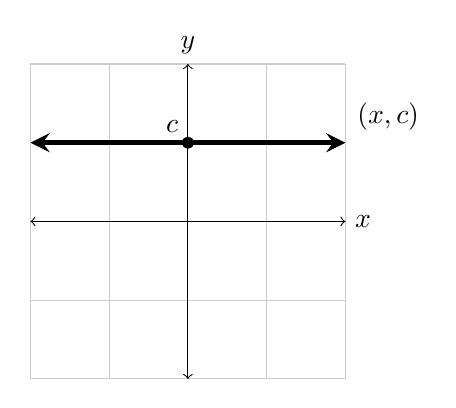
\begin{tikzpicture}
    \draw[thin,gray!40] (-2,-2) grid (2,2);
    \draw[<->] (-2,0)--(2,0) node[right] {$x$};
    \draw[<->] (0,-2)--(0,2) node[above]{$y$};
    \draw[fill=black] (0,1) circle(2pt) node[anchor=south east]{$c$};
    \draw[line width=2pt,black,stealth-stealth] (-2,1)--(2,1) node[anchor=south west]{$(x,c)$};
\end{tikzpicture}
\caption*{Linea horizontal real}
    \end{minipage}
    \begin{minipage}{0.45\textwidth}
        \centering
        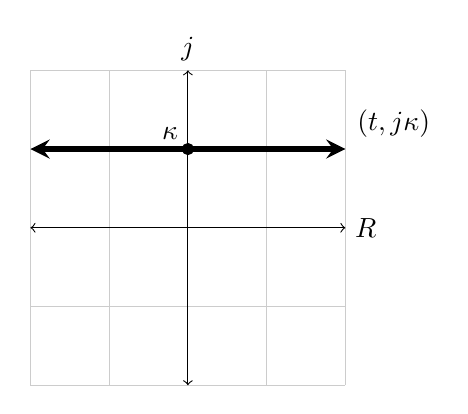
\begin{tikzpicture}
    \draw[thin,gray!40] (-2,-2) grid (2,2);
    \draw[<->] (-2,0)--(2,0) node[right] {$R$};
    \draw[<->] (0,-2)--(0,2) node[above]{$j$};
    \draw[fill=black] (0,1) circle(2pt) node[anchor=south east]{$\kappa$};
    \draw[line width=2pt,black,stealth-stealth] (-2,1)--(2,1) node[anchor=south west]{$(t,j\kappa)$};
\end{tikzpicture}
\caption*{Linea horizontal compleja}
    \end{minipage}
    \caption{}
    \label{fig:ComLHF}
\end{figure}
Restringido los valores que pude tomar $x$ podremos genera segmentos horizontales.

\unsubsubsection{Linea vertical}
En el plano de 2 dimensiones reales una linea vertical es el lugar geométrico en el cual los puntos pertenecientes al mismo posen la misma coordenada constante en $x$, generando una recta perpendicular al eje $y$.
\begin{equation}
    (x,y)\begin{cases}
        y=t\\
        x=c
    \end{cases}
\end{equation}
De manera similar una recta horizontal en el plano complejo esta descripta por la siguiente ecuación:
\begin{equation}\label{eq:DeflvF}
    z=\kappa+jt
\end{equation}
$\kappa$ siendo una constate y $t$ siendo variable.
\begin{figure}[H]
    \centering
    \begin{minipage}{0.45\textwidth}
        \centering
        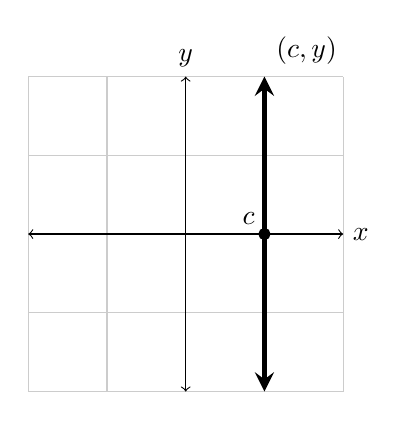
\begin{tikzpicture}
    \draw[thin,gray!40] (-2,-2) grid (2,2);
    \draw[<->] (-2,0)--(2,0) node[right] {$x$};
    \draw[<->] (0,-2)--(0,2) node[above]{$y$};
    \draw[fill=black] (1,0) circle(2pt) node[anchor=south east]{$c$};
    \draw[line width=2pt,black,stealth-stealth] (1,-2)--(1,2) node[anchor=south west]{$(c,y)$};
\end{tikzpicture}
\caption*{Linea vertical real}
    \end{minipage}
    \begin{minipage}{0.45\textwidth}
        \centering
        \input{Plots/FuncionesComplejos/Linea/LineaVF}
    \end{minipage}
    \caption{}
    \label{fig:ComVHF}
\end{figure}
Restringido los valores que pude tomar $y$ podremos genera segmentos verticales.
\unsubsubsection{Rectángulos}
Ahora que definimos como parametrizar lineas horizontales y verticales, podemos crear cuadrados y rectángulos en el plano complejo. Por ejemplo planteamos un rectángulo que tenga por vértices los puntos $\ a=(1+j)$; $\ b=(3+j)$; $\ c=(3+j2)$; $d\ =(1+2j)$, entonces el rectángulo estará conformado por los segmentos horizontales, $\overline{ab}$ y $\overline{cd}$, y los segmentos verticales $\overline{bc}$ y $\overline{da}$. Los segmentos horizontales estarán dados entonces por:
\begin{equation}
\begin{aligned}
    \overline{ab}=(x+jy)&
    \begin{cases}
        x=\Real{a}\leq t\leq\Real{b}\lrah x=1\leq t\leq 3\\
        y=\Imag{a}=\Imag{b}\lrah y=1
    \end{cases}\\
    \\
    \overline{cd}=(x+jy)&
    \begin{cases}
        x= \Real{c}\leq t\leq\Real{d}\lrah x=1\leq t\leq 3\\
        y=\Imag{a}=\Imag{b} \lrah y=2
    \end{cases}
\end{aligned}
\end{equation}
y los segmentos verticales estarán dados por:
\begin{equation}
\begin{aligned}
    \overline{bc}=(x+jy)&
    \begin{cases}
        x=\Real{c}=\Real{d}\lrah x=3\\
        y=\Imag{b}\leq t\leq \Imag{c}\lrah y=1\leq t\leq2
    \end{cases}\\
    \\
    \overline{da}=(x+jy)&
    \begin{cases}
        x=\Real{d}=\Real{a}\lrah x=1\\
        y=\Imag{b}\leq t\leq \Imag{c}\lrah y=1\leq t\leq2
    \end{cases}
\end{aligned}
\end{equation}
Obteniendo la expresión del rectángulo.
\begin{figure}[H]
    \centering
    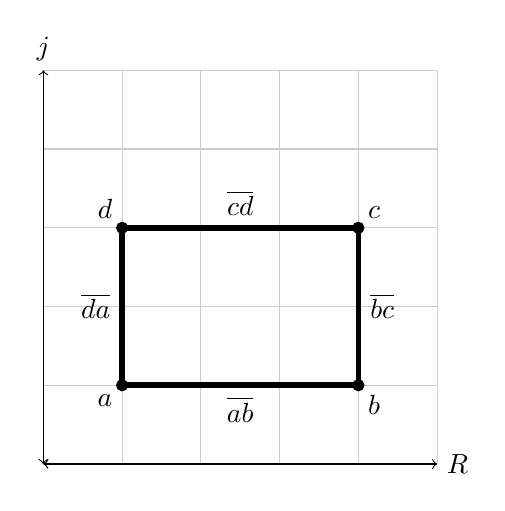
\begin{tikzpicture}
    \draw[thin,gray!40] (0,0) grid (5,5);
    \draw[<->] (0,0)--(5,0) node[right] {$R$};
    \draw[<->] (0,0)--(0,5) node[above]{$j$};
    \coordinate (a) at (1,1);
    \coordinate (b) at (4,1);
    \coordinate (c) at (4,3);
    \coordinate (d) at (1,3);
    
    \draw[fill=black] (a) circle(2pt) node[anchor=north east]{$a$};
    \draw[fill=black] (b) circle(2pt) node[anchor=north west]{$b$};
    \draw[fill=black] (c) circle(2pt) node[anchor=south west]{$c$};
    \draw[fill=black] (d) circle(2pt) node[anchor=south east]{$d$};
    
    \draw[line width=2pt,black,-] (a)--(b) node[midway, below]{$\overline{ab}$};
    \draw[line width=2pt,black,-] (b)--(c) node[midway, right]{$\overline{bc}$};
    \draw[line width=2pt,black,-] (c)--(d) node[midway, above]{$\overline{cd}$};
    \draw[line width=2pt,black,-] (d)--(a) node[midway, left]{$\overline{da}$};
    
\end{tikzpicture}
\caption{Rectángulo en el plano complejo con lineas parametrizadas}
    \label{fig:RectF}
\end{figure}
\unsubsection{Superficies}
Para definir una superficie tomamos como una linea horizontal o vertical, entonces la expresión:
\begin{equation}
    \Real{z} \geq \kappa
\end{equation}
define la superficie $S$ descripta en la figura \ref{fig:SupVF}:
\begin{figure}[H]
    \centering
    \begin{tikzpicture}
    \draw[thin,gray!40] (-2,-2) grid (2,2);
    \draw[<->] (-2,0)--(2,0) node[right] {$R$};
    \draw[<->] (0,-2)--(0,2) node[above]{$j$};
    \filldraw[draw=gray!40, fill=mlgb, fill opacity=0.6] (0.5,-2) -- (0.5,2) -- (2,2) -- (2,-2);
    \draw[line width=2pt,black,-] (0.5,-2)--(0.5,2);
    \draw[fill=black] (0.5,0) circle(2pt) node[anchor=south east]{$\kappa$};
    \draw[] (1.20,0) node[above]{$S$};
\end{tikzpicture}
\caption{Superficie $S$}
    \label{fig:SupVF}
\end{figure}
De manera similar la ecuación:
\begin{equation}
    \Imag{z} \geq \kappa
\end{equation}
define la superficie $S$ de la figura \ref{fig:SupHF}:
\begin{figure}[H]
    \centering
    \begin{tikzpicture}
    \draw[thin,gray!40] (-2,-2) grid (2,2);
    \draw[<->] (-2,0)--(2,0) node[right] {$R$};
    \draw[<->] (0,-2)--(0,2) node[above]{$j$};
    \filldraw[draw=gray!40, fill=mlgb, fill opacity=0.6] (-2,-0.5) -- (2,-0.5) -- (2,2) -- (-2,2);
    \draw[line width=2pt,black,-] (-2,-0.5)--(2,-0.5);
    \draw[fill=black] (0,-0.5) circle(2pt) node[anchor=north east]{$\kappa$};
    \draw[] (0,1.2) node[right]{$S$};
\end{tikzpicture}
\caption{Superficie $S$}
    \label{fig:SupHF}
\end{figure}
\unsubsection{Rectas, semi-rectas y segmentos}
Una recta, en un espacio de 2 dimensiones reales, de ordenada al origen igual al punto $(0,0)$ esta formada por infinitos puntos que satisfagan la condición:
\begin{equation}
   y=x\cdot a \lrah \frac{x}{y}=a
\end{equation}
$a$ siendo una constante arbitraria y $(x\ ,\ y)$ siendo los componentes de los puntos. Si trazamos una linea con cada uno de nuestros punto hasta la ordenada de origen veremos que todas las lineas generan una ángulo de $\tan^{-1}{(\frac{y}{x})}$ con respecto al eje $x$. Ya que $x$ e $y$ son proporcionales entre ellos por un factor $a$, por como se define una recta, todos los puntos poseerán el mismo ángulo con respecto al eje $x$.

En el plano complejo una recta debe comportarse de una manera similar, todos los puntos pertenecientes a la recta deben tener el mismo ángulo o argumento, entonces recordando la definición exponencial de un numero complejo \ref{eq:defExp} podemos definir una recta como un numero complejo de argumento constante $\gamma$ y modulo variable $r$:
\begin{equation}\label{eq:DefRectF}
    z_{(r)}=re^{j\gamma}\llrah \ z_{(r)}=r\cdot[\cos{(\gamma)}+j\sen{(\gamma)}] 
\end{equation}
\begin{figure}[H]%
\centering
    \begin{minipage}{0.5\textwidth}
    \centering
        \input{Plots/FuncionesComplejos/Recta/RectaRF}
    \end{minipage}%
    \begin{minipage}{0.4\textwidth}
    \centering
        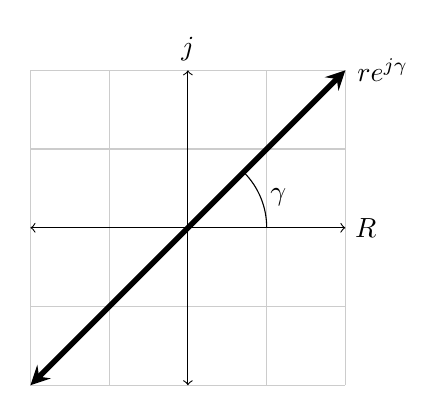
\begin{tikzpicture}
    \draw[thin,gray!40] (-2,-2) grid (2,2);
    \draw[<->] (-2,0)--(2,0) node[right] {$R$};
    \draw[<->] (0,-2)--(0,2) node[above]{$j$};
    \draw[line width=2pt,black,stealth-stealth] plot[smooth,domain=-2:2] (\x, {\x}) node[right]{$re^{j\gamma}$};
    \draw[|-|] (1,0) arc (0:45:1) node [midway, right]{$\gamma$};
\end{tikzpicture}
\caption*{Recta en el plano complejo}
    \end{minipage}%
    \caption{Comparación entre un numero complejo y un vector de 2 dimensiones reales}
    \label{fig:compRectasF}
\end{figure}
En la forma polar de la expresión \ref{eq:DefRectF} se pude ver claramente que, al ser $\gamma$ una constante, el coseno y el seno son también constantes, entonces la parte real e imaginaria siempre van a ser proporcionales a $r$ manteniendo la relación $\frac{\Real{z}}{\Imag{z}}$ constante.
Modificando el intervalo en el que varia $r$ seremos capaces de crear distintos objetos geométricos
\begin{figure}[H]
\centering
    \begin{minipage}{0.3\textwidth}
        \input{Plots/FuncionesComplejos/Recta/RectaINF}
    \end{minipage}
    \begin{minipage}{0.3\textwidth}
        \input{Plots/FuncionesComplejos/Recta/SemirF}
    \end{minipage}
    \begin{minipage}{0.3\textwidth}
        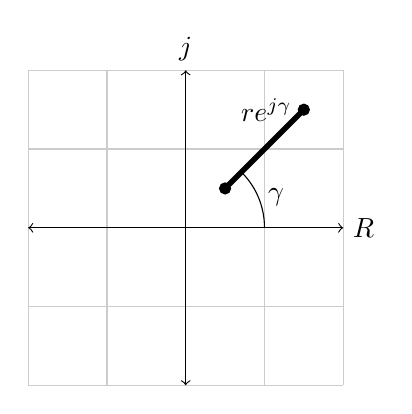
\begin{tikzpicture}
    \draw[thin,gray!40] (-2,-2) grid (2,2);
    \draw[<->] (-2,0)--(2,0) node[right] {$R$};
    \draw[<->] (0,-2)--(0,2) node[above]{$j$};
    \draw [fill=black] (0.5,0.5) circle(2pt);
    \draw [fill=black] (1.5,1.5) circle(2pt);
    \draw[line width=2pt,black,-] plot[smooth,domain=0.5:1.5] (\x, {\x}) node[left]{$re^{j\gamma}$};
    \draw[|-|] (1,0) arc (0:45:1) node [midway, right]{$\gamma$};
\end{tikzpicture}
\caption*{Segmento: $a\leq r \leq b$}
    \end{minipage}
    \caption{}
    \label{fig:RectaExpoF}
\end{figure}
También podemos desplazar la recta sumándole cualquier numero complejo fijo como constante. Entonces la ecuación general de una recta en el plano complejo seria:
\begin{equation}
    z_{(r)}=re^{j\gamma}+z_c \llrah\ z_{(r)}=r\cdot[\cos{(\gamma)}+j\sen{(\gamma)}]+z_c
\end{equation}
\begin{figure}[H]
    \centering
    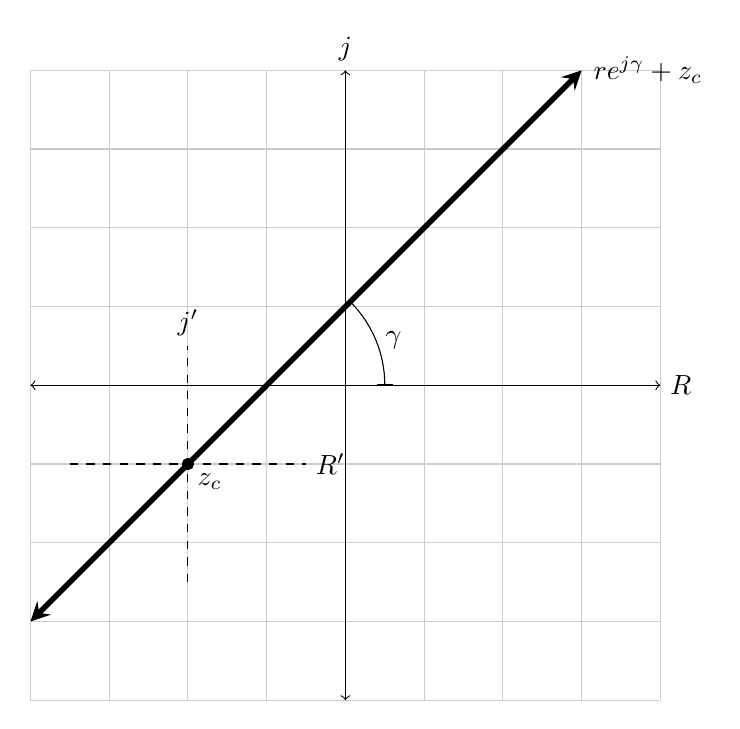
\begin{tikzpicture}
    \draw[thin,gray!40] (-4,-4) grid (4,4);
    \draw[<->] (-4,0)--(4,0) node[right] {$R$};
    \draw[<->] (0,-4)--(0,4) node[above]{$j$};
    \draw[dashed] (-3.5,-1)--(-0.5,-1) node[right] {$R'$};
    \draw[dashed] (-2,-2.5)--(-2,0.5) node[above]{$j'$};
    \draw [fill=black] (-2,-1) circle(2pt) node[anchor=north west]{$z_c$};
    \draw[line width=2pt,black,stealth-stealth] plot[smooth,domain=-4:3] (\x, {\x+1}) node[right]{$re^{j\gamma}+z_c$};
    \draw[|-|] (0.5,0) arc (0:45:1.5) node [midway, right]{$\gamma$};
\end{tikzpicture}
\caption{Recta genérica desplazada un $z_c$}
\end{figure}
Al sumar un numero complejo $z_c$ es como si estuviéramos desplazando los ejes coordenados al punto $z_c$ ya que cuando $r=0$
estaríamos parado en el centro de este nuevo sistema de ejes coordenado desplazado relativamente al antiguo eje coordenado, como si fuera una transformación lineal. La base de este nuevo sistema coordenado seria la base desplazada en $z_c$, $\ j'=j+z_c$ y $\ R'=1+z_c$. Esto ultimo no es muy relevante pero sienta las bases para ver como funciona un desplazamiento en una función compleja.

De la ecuación \ref{eq:DefRectF}, recordando la definición de forma polar \ref{eq:defPol} y sabiendo que $\gamma$ es una constante y por lo tanto el $sin$ y el $cos$ también, podemos desarrollar la expresión:
\begin{equation}
    \begin{aligned}
        z_{(r)}=r\cdot[\cos{(\gamma)}+j\sen{(\gamma)}]+z_c \lrah z_{(r)}&=r\cdot[x_0+jy_0]+z_c\\                                                           z_{(t)}&=t\cdot z_0+z_c
    \end{aligned}
\end{equation}
Entonces una recta no es más que escalar un vector $z_0$ por una variable $t$. Ahora podemos remplazar a $z_0$ por cualquier cosa que represente un vector. Supongamos que queremos representar una linea que pase por 2 puntos del espacio, recordando que la resta describe un vector $\overrightarrow{(z_0z_1)}$ representada en la figura \ref{fig:RestC}:
\begin{equation}\label{eq:RectaCarF}
     z_{(t)}=t\cdot z_0+z_c \lrah z_{(t)}=t\cdot(z_1-z_0)+z_0 \llrah\ z_{(t)}=z_0(1-t)+z_1t
\end{equation}
Esta ecuación representa una recta que es múltiplo del vector $(z_1-z_0)$ y desplazada en $z_0$.
Como vemos en la figura \ref{fig:CartRectF} si no desplazamos la ecuación de la recta \ref{eq:RectaCarF} por $z_0$ la recta no pasara por los puntos $z_0$ y $z_1$. Entonces la ecuación la ecuación \ref{eq:RectaCarF} describe una recta que pasa por los puntos ya mencionados. $t$ pude definirse en términos de intervalos para generar otros objetos geométricos como se describe en la figura \ref{fig:RectaExpoF}.
\begin{figure}[H]
    \centering
    \begin{minipage}{0.4\textwidth}
        \centering
        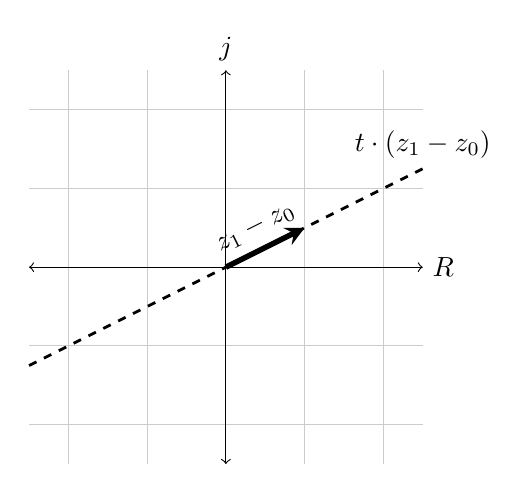
\begin{tikzpicture}
    \draw [thin,gray!40] (-2.5,-2.5) grid (2.5,2.5);
    \draw[<->] (-2.5,0)--(2.5,0) node[right] {$R$};
    \draw[<->] (0,-2.5)--(0,2.5) node[above]{$j$};
    \coordinate (a) at (1,1);
    \coordinate (b) at (3,2);
    \draw[line width=2pt,black,-stealth] (0,0)--(1,0.5) node[midway, above, sloped]{$z_1-z_0$};
    \draw[line width=1pt,black,dashed] (-2.5,-1.25)--(2.5,1.25) node[above]{$t\cdot(z_1-z_0)$};
\end{tikzpicture}
\caption*{Ecuación de la recta sin desplazar}
    \end{minipage}
    \begin{minipage}{0.4\textwidth}
        \centering
        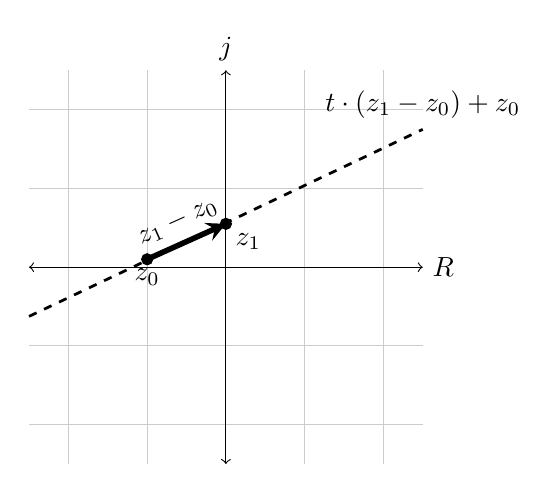
\begin{tikzpicture}
    \draw [thin,gray!40] (-2.5,-2.5) grid (2.5,2.5);
    \draw[<->] (-2.5,0)--(2.5,0) node[right] {$R$};
    \draw[<->] (0,-2.5)--(0,2.5) node[above]{$j$};
    \coordinate (a) at (-1,0.1);
    \coordinate (b) at (-0,0.55);
    \draw[fill=black] (a) circle(2pt) node[below]{$z_0$};
    \draw[fill=black] (b) circle(2pt) node[anchor=north west]{$z_1$};
    \draw[line width=2pt,black,-stealth] (a)--(b) node[midway, above, sloped]{$z_1-z_0$};
    \draw[line width=1pt,black,dashed] (-2.5,-0.625)--(2.5,1.75) node[above]{$t\cdot(z_1-z_0)+z_0$};
\end{tikzpicture}
\caption*{Ecuación de la recta desplazada}
    \end{minipage}
    \caption{Rectas definidas en coordenadas cartesianas}
    \label{fig:CartRectF}
\end{figure}
\unsubsubsection{Triangulo}
Ahora que están todas la herramientas necesarias presentadas construyamos un triangulo que tenga por vértices la coordenadas $\ a=(1,j0)$, $\ b=(3,j2)$, $\ c=(0.5+3j)$. Teniendo los puntos ya definidos y recordando la definición \ref{eq:RectaCarF}:
\begin{equation}
    \overline{z_{ab}}=t\cdot(z_b-z_a)+z_a \lrah\overline{z_{ab}}=t\cdot(2+2j)+1
    \begin{cases}
        t\therefore\overline{z_{ab}}=z_a\lrah t=0\\
        t\therefore\overline{z_{ab}}=z_b\lrah t=1\\
    \end{cases}
\end{equation}
Para la recta $\overline{z_{ab}}$, $t$ va a existir en el intervalo $0\leq t\leq1$ ya que cundo $t=1$ $\overline{z_{ab}}=z_b$ y cuando $t=0$ $\overline{z_{ab}}=z_a$. Se realiza el mismo analisis para las rectas $\overline{z_{bc}}$ y $\overline{z_{ca}}$
\begin{equation}
    \overline{z_{bc}}=t\cdot(z_c-z_b)+z_b \lrah\overline{z_{bc}}=t\cdot(-2.5+1j)+(3+j2)
    \begin{cases}
        0\leq t\leq1
    \end{cases}
\end{equation}
\begin{equation}
    \overline{z_{ca}}=t\cdot(z_a-z_c)+z_c \lrah\overline{z_{bc}}=t\cdot(0.5-3j)+(0.5+j3)
    \begin{cases}
         0\leq t\leq1
    \end{cases}
\end{equation}
\begin{figure}[H]
    \centering
    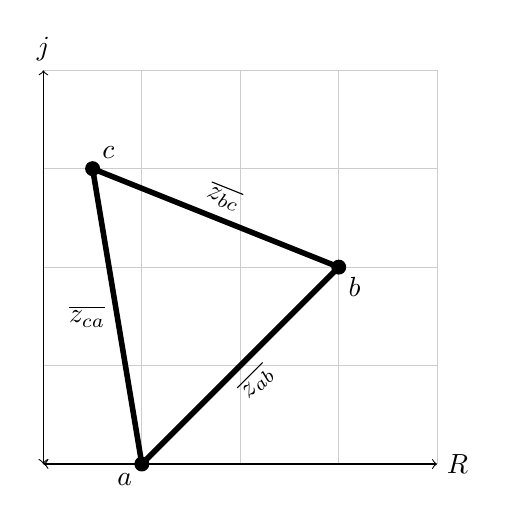
\begin{tikzpicture}[scale=1.25]
    \draw[thin,gray!40] (0,0) grid (4,4);
    \draw[<->] (0,0)--(4,0) node[right] {$R$};
    \draw[<->] (0,0)--(0,4) node[above]{$j$};
    \coordinate (a) at (1,0);
    \coordinate (b) at (3,2);
    \coordinate (c) at (0.5,3);
    
    \draw[fill=black] (a) circle(2pt) node[anchor=north east]{$a$};
    \draw[fill=black] (b) circle(2pt) node[anchor=north west]{$b$};
    \draw[fill=black] (c) circle(2pt) node[anchor=south west]{$c$};
    
    \draw[line width=2pt,black,-] (a)--(b) node[midway, below, sloped]{$\overline{z_{ab}}$};
    \draw[line width=2pt,black,-] (b)--(c) node[midway, above, sloped ]{$\overline{z_{bc}}$};
    \draw[line width=2pt,black,-] (c)--(a) node[midway, left]{$\overline{z_{ca}}$};
    
\end{tikzpicture}
\caption{Triangulo en el plano complejo con rectas parametrizadas}
    \label{fig:TrianCF}
\end{figure}

\unsubsection{Circunferencias, arcos, discos y segmentos de disco}
En el plano de 2 dimensiones una circunferencia es el lugar geométrico en el cual todos los punto pertenecientes al mismo tiene un distancia constante $r$ respecto a un punto $(a,b)$ de referencia llamado centro.
\begin{equation}\label{eq:DefCircR}
    \begin{aligned}
       (x-a)^2+(y-b)^2=r^2 \lrah \sqrt{(x-a^2+(y-b)^2}=&r \\
       |(x-a,y-b)|=&r
    \end{aligned}
\end{equation} 
Como podemos ver la ecuación \ref{eq:DefCircR} describe un modulo constante de valor $r$, esto en el plano complejo es fácil de definir, recordando las definiciones de la forma polar\ref{eq:defPol} y exponencial\ref{eq:defExp} dejando el modulo $r$ como una constante y dejamos el argumento como un  parámetro. Recordando que el argumento de un numero complejo esta definido como $-\pi<\theta\leq\pi$:
\begin{equation}\label{eq:ParamcircF}
    z=re^{j\theta}+z_0 \llrah\ z=r[\cos{(\theta)}+j\sen{(\theta)}]+z_0
\end{equation}
\begin{equation}
    re^{j\theta}
    \begin{cases}
        r=\kappa\\
        -\pi<\theta\leq\pi
    \end{cases}
\end{equation}
\begin{figure}[H]
    \centering
    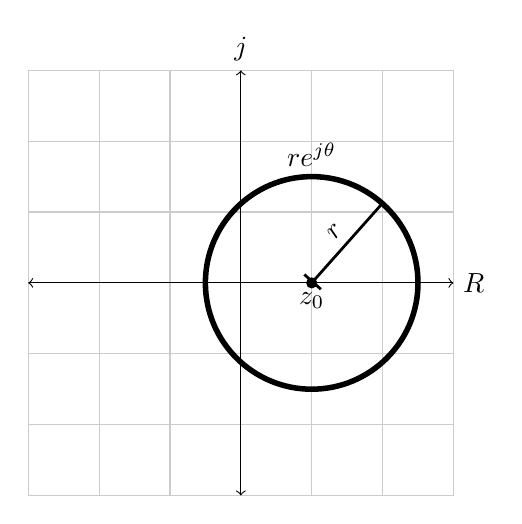
\begin{tikzpicture} [scale=0.9]
    \draw[thin,gray!40] (-3,-3) grid (3,3);
    \draw[<->] (-3,0)--(3,0) node[right] {$R$};
    \draw[<->] (0,-3)--(0,3) node[above]{$j$};
    \draw[line width=2pt] (1,0) circle(1.5);
    \draw[] (1,1.5) node[above]{$re^{j\theta}$};
    \draw[fill=black] (1,0) circle(2pt) node[below]{$z_0$};
    \draw[line width=1pt,black,|-|] (1,0)--(2,1.125) node[midway,above,sloped]{$r$};
\end{tikzpicture}
\caption{Circunferencia en el plano complejo de centro $z_0$}
    \label{fig:CircCF}
\end{figure}
Restringiendo el intervalo en el que existe el argumento podremos crear un arco. Un ejemplo seria $-\frac{\pi}{4}\leq\theta\leq\frac{\pi}{4}$:
\begin{equation}
    re^{j\theta}+z_0
    \begin{cases}
        r=\kappa\\
        -\frac{\pi}{4}\leq\theta\leq\frac{\pi}{4}
    \end{cases}
\end{equation}
\begin{figure}[H]
    \centering
    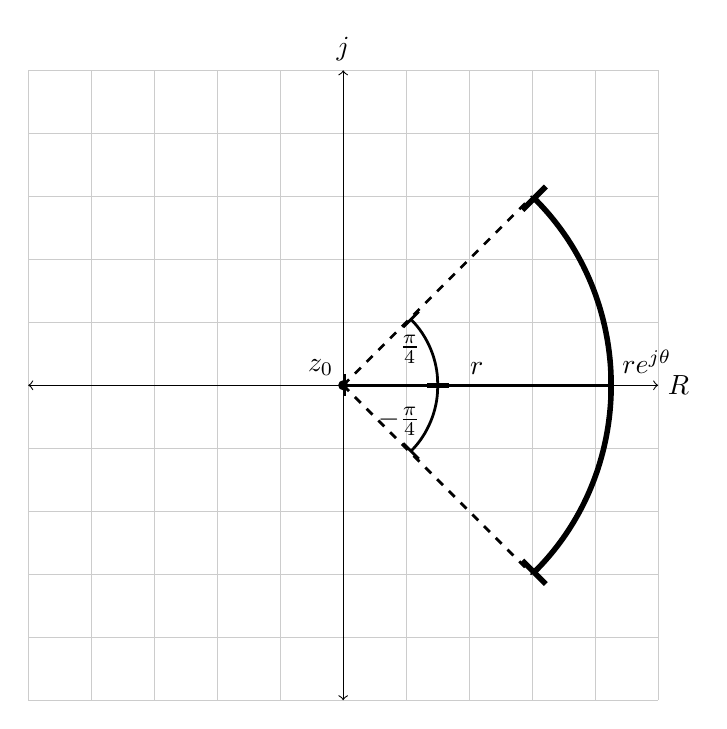
\begin{tikzpicture}[scale=0.8]
    \draw[thin,gray!40] (-5,-5) grid (5,5);
    \draw[<->] (-5,0)--(5,0) node[right] {$R$};
    \draw[<->] (0,-5)--(0,5) node[above]{$j$};
    \draw[line width=2pt,black,|-|] (3,-3) arc (-45:45:4.2426) node [midway,anchor=south west]{$re^{j\theta}$};
    \draw[line width=1pt,black,|-|] (1.5,0) arc (0:45:1.5) node [midway, left]{$\frac{\pi}{4}$};
    \draw[line width=1pt,black,|-|] (1.5,0) arc (0:-45:1.5) node [midway, left]{$-\frac{\pi}{4}$};
    \draw[fill=black] (0,0) circle(2pt) node[anchor=south east]{$z_0$};
    \draw[line width=1pt,black,dashed] (0,0)--(3,3);
    \draw[line width=1pt,black,dashed] (0,0)--(3,-3);
    \draw[line width=1pt,black,|-|] (0,0)--(4.2426,0) node[midway,above,sloped]{$r$};

  
\end{tikzpicture}
\caption{Arco en el plano complejo de centro $z_0$}
    \label{fig:ArcCF}
\end{figure}

Ahora si además de variar el argumento sin restringirlo y asociamos a $r$ con intervalo del tipo $r_0\leq r\leq r_1$ generaremos un disco de radio interior $r_0$ y radio exterior $r_1$:
\begin{equation}
    re^{j\theta}+z_0
    \begin{cases}
        r_0\leq r\leq r_1\\
        -\pi<\theta\leq\pi
    \end{cases}
\end{equation}
\begin{figure}[H]
    \centering
    \begin{tikzpicture}
    \draw[thin,gray!40] (-4,-4) grid (4,4);
    \draw[<->] (-4,0)--(4,0) node[right] {$R$};
    \draw[<->] (0,-4)--(0,4) node[above]{$j$};
    \fill[fill=mlgb, fill opacity=0.6,even odd rule] (0,0) circle (3) (0,0) circle (1);
    \draw[fill=black] (0,0) circle(2pt) node[anchor=north east]{$z_0$};
    \draw[line width=1pt,|-|] (0,0) -- (0.707,0.707) node[midway,above,sloped]{$r_0$};
    \draw[line width=1pt,|-|] (0,0) -- (-2.1213,2.1213) node[midway,above,sloped]{$r_1$};
    \draw [black,line width=2pt](0, 0) circle (1);
    \draw [black,line width=2pt](0, 0) circle (3);
\end{tikzpicture}
\caption{Disco en el plano complejo}
    \label{fig:DiscoCF}
\end{figure}
Conociendo todo esto y además recordando la definición de rectas en el plano complejo \ref{eq:RectaCarF} se podrá definir un segmento de disco. Planteando un ejemplo en el cual los vértices del segmento sean $a=(1,j0.5)$, $\ b=(3+j0.5)$, $\ c=(1.521+j3.512)$ y $\ d=(0.559+j1.291)$. Como vemos nuestro segmento estará conformado por una linea horizontal $\ \overline{ab}$, dos arcos $\ \vec{bc}$, $\ \Vec{da}$ y una recta $\overline{z_{cd}}$.
\begin{equation}
    \overline{ab}=(t+j\kappa)\lrah
    \begin{cases}
        \kappa=0.5\\
        1\leq t\leq3
    \end{cases}
\end{equation}
\begin{equation}
    \overline{z_{cd}}=t\cdot(z_c-z_d)+z_d \lrah\overline{z_{cd}}=t\cdot(0.962+2.221j)+(0.559+j1.291)
    \begin{cases}
         0\leq t\leq1
    \end{cases}
\end{equation}
El arco $\vec{bc}$ debe tener necesariamente el mismo modulo que los puntos por donde pasa y el argumento debe variar en un intervalo desde el argumento del punto inicial hasta el argumento del punto final.
\begin{equation}
    \vec{bc}=re^{j\theta}
    \begin{cases}
        \tan^{-1}{\frac{\Imag{b}}{\Real{b}}}\leq\theta\leq\tan^{-1}{\frac{\Imag{c}}{\Real{z_c}}}\lrah0.052\pi\leq\theta\leq0.367\pi\\
        \\
        r=|c|=|b|=3.04
    \end{cases}
\end{equation}
\begin{equation}
    \vec{da}=re^{j\theta}
    \begin{cases}
        \tan^{-1}{\frac{\Imag{a}}{\Real{a}}}\leq\theta\leq\tan^{-1}{\frac{\Imag{d}}{\Real{d}}}\lrah0.148\pi\leq\theta\leq0.367\pi\\
        \\
        r=|d|=|a|=1.18
    \end{cases}
\end{equation}
\begin{figure}[H]
    \centering
    \begin{tikzpicture}[scale=1.5]
    \draw[thin,gray!40] (0,0) grid (4,4);
    \draw[<->] (0,0)--(4,0) node[right] {$R$};
    \draw[<->] (0,0)--(0,4) node[above]{$j$};
    \coordinate (a) at (1,0.5);
    \coordinate (b) at (3,0.5);
    \coordinate (c) at (1.521,2.634);
    \coordinate (d) at (0.559,1.022);
    
    \fill[fill=mlgb,opacity=0.6,even odd rule](a)--(b) arc (9.4623:60:3.0414)--(0.54,1.022) arc (60:26.56505:0.8)--(a) ;
    
    \draw[fill=black] (a) circle(2pt) node[anchor=north]{$a$};
    \draw[fill=black] (b) circle(2pt) node[anchor=north]{$b$};
    \draw[fill=black] (c) circle(2pt) node[anchor=south]{$c$};
    \draw[fill=black] (d) circle(2pt) node[anchor=east]{$d$};
    
    \draw[line width=2pt,black,-] (a)--(b) node[midway, below]{$\overline{ab}$};
    \draw[line width=2pt,black,-] (b) arc (9.4623:60:3.0414) node [midway,anchor=south west]{$\Vec{bc}$};
    \draw[line width=2pt,black,-] (c)--(d) node[midway, above,sloped]{$\overline{cd}$};
    \draw[line width=2pt,black,-] (a) arc (26.56505:60:1.18) node [midway,anchor=north east]{$\Vec{da}$};

    
    
\end{tikzpicture}
\caption{Segmento de disco en el plano complejo con lineas parametrizadas}
    \label{fig:SegDiscCF}
\end{figure}

Podemos plantear otro ejemplo con los puntos a $a=(1,j)$, $b=(2,j2)$, $c=(-1,j)$ y $d=(-2,2j)$ como vemos el segmento del disco estará conformado por las rectas $\overline{ab}$, $\overline{cd}$ y los arcos $\vec{bc}$, $\vec{da}$:
\begin{equation}
    \begin{aligned}
        \overline{ab}&=t\cdot(z_b-z_a)+z_a
        \begin{cases}
        \overline{ab}=t\cdot(1+j)+(1+j) \llrah\ re^{j\frac{\pi}{4}}\\
            0\leq t\leq 1 \llrah\ 1\leq r\leq 2
        \end{cases}\\
        \\
        \overline{cd}&=t\cdot(z_d-z_c)+z_c 
        \begin{cases}
        \overline{cd}=t\cdot(-1+j)+(-1+j) \llrah\ re^{j\frac{4\pi}{3}}\\
            0\leq t\leq 1 \llrah\ 1\leq r\leq 2
        \end{cases}\\
    \end{aligned}
\end{equation}
\begin{equation}
    \begin{aligned}
     \vec{bd}&=re^{j\theta}
    \begin{cases}
       \frac{\pi}{4}\leq\theta\leq\frac{4\pi}{3}\\
        \\
        r=|c|=|b|=2
    \end{cases}\\
     \vec{ca}&=re^{j\theta}
    \begin{cases}
       \frac{\pi}{4}\leq\theta\leq\frac{4\pi}{3}\\
        \\
        r=|d|=|a|=1
    \end{cases}
    \end{aligned}
\end{equation}
\begin{figure}[H]
    \centering
    \begin{tikzpicture}
    \draw[thin,gray!40] (-5,0) grid (5,6);
    \draw[<->] (-5,0)--(5,0) node[right] {$R$};
    \draw[<->] (0,0)--(0,6) node[above]{$j$};
    \coordinate (a) at (1,1);
    \coordinate (b) at (3,3);
    \coordinate (c) at (-1,1);
    \coordinate (d) at (-3,3);
    \fill[fill=mlgb,opacity=0.6,even odd rule](a)--(b) arc (45:135:4.2426)--(c)  arc (135:45:1.4142)--(a) ;
    
    \draw[fill=black] (a) circle(2pt) node[anchor=north west]{$a$};
    \draw[fill=black] (b) circle(2pt) node[anchor=south west]{$b$};
    \draw[fill=black] (c) circle(2pt) node[anchor=north east]{$c$};
    \draw[fill=black] (d) circle(2pt) node[anchor=south east]{$d$};
    
    \draw[line width=2pt,black,-] (a)--(b) node[midway, right]{$\overline{ab}$};
    \draw[line width=2pt,black,-] (c)--(d) node[midway, left]{$\overline{cd}$};
    \draw[line width=2pt,black,-] (b) arc (45:135:4.2426) node [midway,above]{$\Vec{bc}$};
    \draw[line width=2pt,black,-] (a) arc (45:135:1.4142) node [midway,below]{$\Vec{da}$};
    
\end{tikzpicture}
\caption{Segmento de disco en el plano complejo con lineas parametrizadas}
    \label{fig:SegDiscCF2}
\end{figure}

\unsection{Funciones complejas}
Un función compleja rige el comportamiento de el plano complejo en su totalidad y transforma números complejos a números complejos. Se podría decir que una función compleja toma el plano complejo $z$ y lo transforma en otro plano complejo $w$. 
Una función compleja se define de la siguiente manera:
\begin{equation}
    f(z)=w
\end{equation}
\begin{figure}[H]
\centering
    \begin{minipage}{0.4\textwidth}
    \centering
       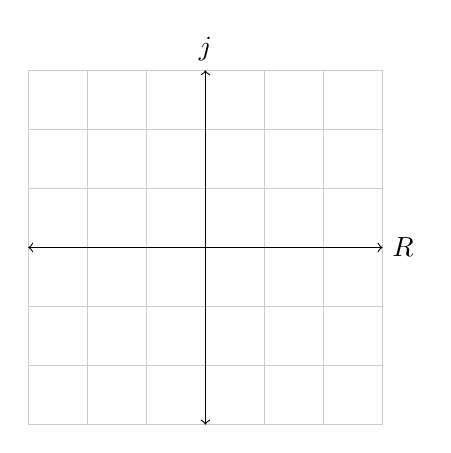
\begin{tikzpicture}[scale= 0.75]
        \draw[thin,gray!40] (-3,-3) grid (3,3);
        \draw[<->] (-3,0)--(3,0) node[right] {$R$};
        \draw[<->] (0,-3)--(0,3) node[above]{$j$};
\end{tikzpicture}
\caption*{Plano complejo $z$}
    \label{fig:PlanoCF1}
    \end{minipage}%
    \begin{minipage}[t]{0.2\textwidth}
        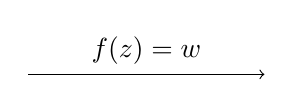
\begin{tikzpicture}
        \centering
            \draw[->] (0,0)--(3,0) node[midway, above] {$f(z)=w$};
        \end{tikzpicture} 
    \end{minipage}%
   \begin{minipage}{0.4\textwidth}
    \centering
       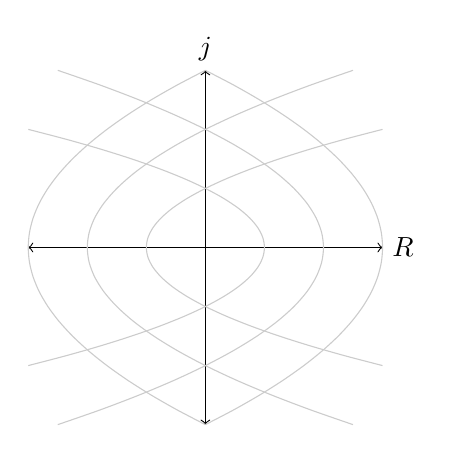
\begin{tikzpicture}[scale= 0.75]
        \draw[<->] (-3,0)--(3,0) node[right] {$R$};
        \draw[<->] (0,-3)--(0,3) node[above]{$j$};
        \draw[rotate=90,thin,gray!40]   plot[smooth,domain=-2:2] (\x, {((\x)^2)-1});
        \draw[rotate=90,thin,gray!40]   plot[smooth,domain=-3:3] (\x, {((\x)^2)/2-2});
        \draw[rotate=90,thin,gray!40]   plot[smooth,domain=-3:3] (\x, {((\x)^2)/3-3});
        \draw[rotate=-90,thin,gray!40]   plot[smooth,domain=-2:2] (\x, {((\x)^2)-1});
        \draw[rotate=-90,thin,gray!40]   plot[smooth,domain=-3:3] (\x, {((\x)^2)/2-2});
        \draw[rotate=-90,thin,gray!40]   plot[smooth,domain=-3:3] (\x, {((\x)^2)/3-3});
\end{tikzpicture}
\caption*{Plano complejo $w$}
    \label{fig:PlanoCF2}
    \end{minipage}%
    \caption{}
    \label{fig:CompPLF}
\end{figure}
La convención es que la variable independiente se la llame $\ z=x+jy$ y la dependiente $\ w=u+jv$. Como en el caso de las ecuaciones una función compleja también se puede sub dividir en 2 partes, una que rija la parte real y otra que rija la parte imaginaria.Para visualizar como funcionan las funciones complejas se utiliza el mapeo de curvas parametrizadas como herramienta.

El concepto del mapeo es tomar una curva y ver como seria transformada en el plano $w$ aplicándole la función únicamente a la curva y graficarlo sobre el plano $z$, como si estuviéramos tomando una muestra del plano complejo $w$.
\unsubsection{Desplazamiento}
Un desplazamiento en el plano complejo se define con la forma de:
\begin{equation}\label{eq:defDespF}
    w=z+z_0
\end{equation}
Siendo $z_0$ un numero complejo, esta función desplaza todo los puntos del plano $z$ en $z_0$. Viendo como se modifica la parte real y parte imaginaria queda implicito el desplazamiento:
\begin{equation}
    w=z+z_0\lrah(u+jv)=(x+jy)+(x_0+jy_0)
    \begin{cases}
        u=x+x_0\\
        v=y+y_0
    \end{cases}
\end{equation}
Para ver gráficamente como se mapea el plano $z$ en el plano $w$, plantemos un rectángulo en el plano $z$ y le apliquemos la función desplazamiento:
\begin{equation}\label{eq:EjemDespF}
    w=z+z_0\lrah w=z+(1+j)    
\end{equation}
por ejemplo. 

El rectángulo $S$ en el plano $z$ sera  el del ejemplo de la figura \ref{fig:RectF}. Recordemos que los puntos que define al rectángulos en el plano $z$ son $\ a=(1+j)$, $\ b=(3+j)$, $\ c=(3+j2)$ y $d\ =(1+2j)$ entonces en el plano $z$, el rectángulo, esta descripto por las ecuaciones:
\begin{equation}
    \begin{aligned}
        \overline{ab}&=(t+j);\  1\leq t\leq3;\\
        \overline{cd}&=(t+j2);\  1\leq t\leq3;\\
        \overline{bc}&=(3+jt);\  1\leq t\leq2;\\
        \overline{da}&=(1+jt);\  1\leq t\leq2;
    \end{aligned}
\end{equation}
Aplicando la función desplazamiento\ref{eq:EjemDespF} a las ecuaciones:
\begin{equation}
    \begin{aligned}
         f_{(\overline{ab})}&=(t+j)+(1+j)  \lrah\ \overline{ab}'=(t+1)+j2\ ;\  1\leq t\leq3;\\
         f_{(\overline{cd})}&=(t+j2)+(1+j) \lrah \overline{cd}'=(t+1)+j3\ ;\  1\leq t\leq3;\\
         f_{(\overline{bc})}&=(3+jt)+(1+j) \lrah \overline{bc}'=4+j(t+1)\ ;\  1\leq t\leq2;\\
         f_{(\overline{da})}&=(1+jt)+(1+j) \lrah \overline{da}'=2+j(t+1)\ ;\  1\leq t\leq2;
    \end{aligned}
\end{equation}
Haciendo un cambio de variable $t'=(t+1)$ quedarían definidos como:
\begin{equation}
    \begin{aligned}
        &\overline{ab}'=t'+j2\ ;\  2\leq t'\leq4;\\
        &\overline{cd}'=t'+j3\ ;\  2\leq t'\leq4;\\
        &\overline{bc}'=4+jt'\ ;\  2\leq t'\leq3;\\
        &\overline{da}'=2+jt'\ ;\  2\leq t'\leq3;
    \end{aligned}
\end{equation}
\begin{figure}[H]
    \centering
    \begin{minipage}{0.39\textwidth}
    \centering
        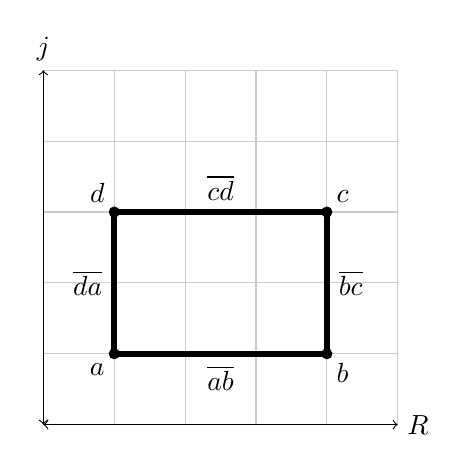
\begin{tikzpicture}[scale=0.9]
    \draw[thin,gray!40] (0,0) grid (5,5);
    \draw[<->] (0,0)--(5,0) node[right] {$R$};
    \draw[<->] (0,0)--(0,5) node[above]{$j$};
    \coordinate (1) at (1,1);
    \coordinate (2) at (4,1);
    \coordinate (3) at (4,3);
    \coordinate (4) at (1,3);
    
    \draw[fill=black] (1) circle(2pt) node[anchor=north east]{$a$};
    \draw[fill=black] (2) circle(2pt) node[anchor=north west]{$b$};
    \draw[fill=black] (3) circle(2pt) node[anchor=south west]{$c$};
    \draw[fill=black] (4) circle(2pt) node[anchor=south east]{$d$};
    
    \draw[line width=2pt,black,-] (1)--(2) node[midway, below]{$\overline{ab}$};
    \draw[line width=2pt,black,-] (2)--(3) node[midway, right]{$\overline{bc}$};
    \draw[line width=2pt,black,-] (3)--(4) node[midway, above]{$\overline{cd}$};
    \draw[line width=2pt,black,-] (4)--(1) node[midway, left]{$\overline{da}$};
    
\end{tikzpicture}
\caption*{Rectángulo $s$}

    \end{minipage}
    \begin{minipage}[t]{0.2\textwidth}
    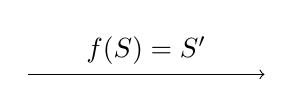
\begin{tikzpicture}
        \centering
            \draw[->] (0,0)--(3,0) node[midway, above] {$f(S)=S'$};
        \end{tikzpicture} 
    \end{minipage}
    \begin{minipage}{0.39\textwidth}
    \centering
        \input{Plots/FuncionesComplejos/Mappeo/Lineal/DespF2}
    \end{minipage}
    \caption{}
\end{figure}
Podemos graficar el plano $w$ en el plano $z$ para denotar como el la función desplazamiento mueve el plano complejo.
\begin{figure}[H]
    \centering
    \begin{tikzpicture}[scale=1.5]
    \draw[thin,gray!40] (0,0) grid (5,5);
    \draw[mlgb,line width=1pt, ->] (0,0)--(5,0) node[right] {$R$};
    \draw[mlgb,line width=1pt, ->] (0,0)--(0,5) node[above]{$j$};
    \draw[line width=1pt, <->] (0,1)--(5,1) node[right] {$R'$};
    \draw[line width=1pt, <->] (1,0)--(1,5) node[above]{$j'$};
    \coordinate (1) at (1,1);
    \coordinate (2) at (4,1);
    \coordinate (3) at (4,3);
    \coordinate (4) at (1,3);
    \coordinate (a) at (2,2);
    \coordinate (b) at (5,2);
    \coordinate (c) at (5,4);
    \coordinate (d) at (2,4);
    
    \draw[fill=black] (1) circle(2pt) node[anchor=south east]{$z_0$} node[mlgb,anchor=north west]{$a$};
    \draw[mlgb,fill=mlgb] (2) circle(1pt) node[anchor=north west]{$b$};
    \draw[mlgb,fill=mlgb] (3) circle(1pt) node[anchor=south east]{$c$};
    \draw[mlgb,fill=mlgb] (4) circle(1pt) node[anchor=south east]{$d$};
    
    \draw[fill=black] (a) circle(2pt) node[anchor=north west]{$a'$};
    \draw[fill=black] (b) circle(2pt) node[anchor=north]{$b'$};
    \draw[fill=black] (c) circle(2pt) node[anchor=south east]{$c'$};
    \draw[fill=black] (d) circle(2pt) node[anchor=south east]{$d'$};
    
    \draw[line width=1pt,mlgb,dashed] (1)--(2) node[midway, below]{$\overline{ab}$};
    \draw[line width=1pt,mlgb,-] (2)--(3) node[midway, right]{$\overline{bc}$};
    \draw[line width=1pt,mlgb,-] (3)--(4) node[midway, above]{$\overline{cd}$};
    \draw[line width=1pt,mlgb,dashed] (4)--(1) node[midway, left]{$\overline{da}$};
    
    \draw[line width=2pt,black,-] (a)--(b) node[midway, below]{$\overline{ab}'$};
    \draw[line width=2pt,black,-] (b)--(c) node[midway, right]{$\overline{bc}'$};
    \draw[line width=2pt,black,-] (c)--(d) node[midway, above]{$\overline{cd}'$};
    \draw[line width=2pt,black,-] (d)--(a) node[midway, left]{$\overline{da}'$};

    \draw[line width=2pt,black, -stealth] (0,0)--(1) node[midway, left]{};
    \draw[line width=1pt,black,dotted] (1)--(a) node[midway, left]{};
    \draw[line width=1pt,black,dotted] (3)--(c) node[midway, left]{};
    \draw[line width=1pt,black,dotted] (2)--(b) node[midway, left]{};
    \draw[line width=1pt,black,dotted] (4)--(d) node[midway, left]{};
    
\end{tikzpicture}
\caption{Plano $w$ graficado sobre el plano $z$ siendo $f_z$ un desplazamiento}
    \label{fig:DespZWF}
\end{figure}
Como se pude interpretar en la figura \ref{fig:DespZWF} cualquier curva parametrizada ahora estará desplazada en $z_0$, recordando la parametrizaciones las curvas dadas en \ref{eq:ParamcircF} y \ref{eq:RectaCarF}, rectas y circunferencias se mapean en:
\begin{equation}
    f_{(z)}=z+z_0
    \begin{cases}
        f_{(z)}=[t\cdot(z_a-z_b)+z_c]+z_0 \lrah f_{(z)}=t\cdot(z_a-z_b)+(z_c+z_0)\\
        f_{(z)}=[re^{j\theta}+z_c]+z_0 \lrah  f_{(z)}=re^{j\theta}+(z_c+z_0)
    \end{cases}
\end{equation}
Entonces el desplazamiento modifica los centros de las circunferencia-arcos y la ordenada al origen de las rectas.

\unsubsection{Escalado}
La función escaldo se define como:
\begin{equation}
    w=\lambda\cdot z
\end{equation}
$\lambda$ siendo un numero real. 
Planteando un numero complejo de la forma $z=re^{j\theta}$ y $z=(a+jb)$ podemos ver que la función escalado se comporta como:
\begin{equation}
    w=\lambda z
    \begin{cases}
        w=\lambda\cdot (re^{j\theta})\lrah w=(\lambda r)e^{j\theta}\\
        w=\lambda\cdot(a+jb)\lrah w=(\lambda a)+j(\lambda b) 
    \end{cases}
\end{equation}
Recordando las propiedades del operador $||$, vemos que la función escalado no modifico el argumento del numero complejo solo escala el modulo por un factor $\lambda$. Separando la expresión en su parte real e imaginaria se ve que ambas partes están escaladas por el mismo factor:
\begin{equation}
    w=\lambda z\lrah (u+jv)=\lambda(x+jy)
    \begin{cases}
        u=\lambda x
        v=\lambda y
    \end{cases}
\end{equation}
Plantemos un disco, un segmento de recta y una recta para apreciar como se modifican el plano $w$ con respecto al $z$:
\begin{equation}
    \begin{aligned}
        \vec{a}=&re^{j\theta}+z_c\lrah 1e^{j\theta}+(-1+j)\\
         z_0=&t(z_a-z_b)+z_b\lrah t(1+j)+2\llrah\ te^{j\frac{\pi}{4}}+2\begin{cases}
            1\leq t\leq\ 2
    \end{cases}\\
        z_1=&t(z_c-z_d)+z_b\lrah t(1.376+j)\llrah\ te^{j\frac{\pi}{5}}\begin{cases}
            -\infty\leq t\leq\infty
    \end{cases}
    \end{aligned}
\end{equation}
Aplicando les un escalado de $\lambda=2$ las expresiones quedarían como:
\begin{equation}
    \begin{aligned}
        f_{(\Vec{a})}=&\lambda (2e^{j\theta}+(-1-j))\lrah 4e^{j\theta}+(-2-j2)\\
        f_{(z_0)}=&\lambda(t(1+j)+2)\lrah w_0=2t(1+j)+4\llrah\ 2te^{j\frac{\pi}{4}}+4\begin{cases}
            1\leq t\leq\ 2
    \end{cases}\\
        f_{(z_1)}=&\lambda(t(1.376+j)) \lrah w_1=2t(1.376+j)\llrah\ 2te^{j\frac{\pi}{5}}\begin{cases}
            -\infty\leq t\leq\infty
    \end{cases}
    \end{aligned}
\end{equation}
Haciendo un cambio de variable $t'=2t$, las expresiones del segmento de recta y la recta quedarían de la siguiente manera:
\begin{equation}
    \begin{aligned}
        w_0=&2t(1+j)+4\begin{cases}
            1\leq t\leq\ 3
    \end{cases}\lrah w_0=t'(1+j)+4\begin{cases}
            2\leq t'\leq\ 4
    \end{cases}\\
        w_1=& 2t(1.376+j)\begin{cases}
            -\infty\leq t\leq\infty
        \end{cases}\lrah w_1=t'(1.376+j)\begin{cases}
            -\infty\leq t'\leq\infty
        \end{cases}
    \end{aligned}
\end{equation}
El escalamiento modifico la ordenada al origen de la recta $z_0$ y el centro de la circunferencia $\Vec{a}$, multiplicando ambos puntos por $\lambda$.Entonces podemos decir que los objetos mapeados que tengan por centro el punto $(0,j0)$ en el plano $z$ no se veran desplazados y su centro sera el mismo. Si los objetos sufren de un desplazamiento en $z_c$ en el plano $z$, se verán desplazados $\lambda z_c$ en el plano $w$.

También vemos el escalamiento modifica la extensión de los intervalos acotados, en este ejemplo pasamos de un intervalo de modulo 1 a un intervalo de modulo 2. Otra forma de interpretarlo es que el escalado, en el caso de las rectas aumenta el tamaño del modulo del vector $(z_0-z_1)$ que describe la recta, en vez de modificar la longitud de los intervalos del parámetro $t$. Recordemos la definición de una recta que pasa por 2 puntos \ref{eq:RectaCarF}:
\begin{equation}
    \begin{aligned}
        f_{(z_0)}=&\lambda(t(1+j)+2)\lrah w_0=t(2+j2)+4\begin{cases}
            1\leq t\leq\ 2
    \end{cases}\\
        f_{(z_1)}=&\lambda(t(1.376+j)) \lrah w_1=t(2.752+j2) \begin{cases}
            -\infty\leq t\leq\infty
    \end{cases}
    \end{aligned}
\end{equation}
\begin{figure}[H]
    \centering
    \begin{minipage}{0.39\textwidth}
         \input{Plots/FuncionesComplejos/Mappeo/Lineal/EscaF1}
    \end{minipage}
     \begin{minipage}{0.2\textwidth}
    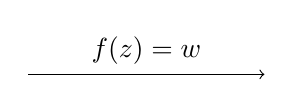
\begin{tikzpicture}
        \centering
            \draw[->] (0,0)--(3,0) node[midway, above] {$f(z)=w$};
        \end{tikzpicture} 
    \end{minipage}
    \begin{minipage}{0.39\textwidth}
         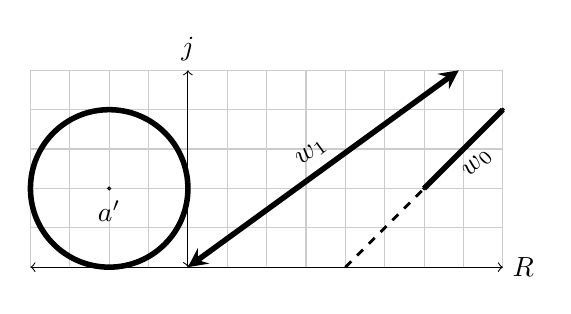
\begin{tikzpicture}[scale=0.5]
    \draw [thin,gray!40] (-4,0) grid (8,5);
    \draw[<->] (-4,0)--(8,0) node[right] {$R$};
    \draw[<->] (0,0)--(0,5) node[above]{$j$};
    \coordinate (a) at (-2,2);
    \coordinate (b) at (6,2);
    \coordinate (c) at (8,4);
    \coordinate (d) at (-5,-3.634);
    \coordinate (e) at (6.88,5);
    \coordinate (f) at (4,0);
    
    \draw[line width=2pt,black] (a) circle(2) node[anchor=north]{$\Vec{a'}$};
    \draw[black] (a) circle(1pt) node[anchor=south]{};
    \draw[black] (b) circle(1pt) node[anchor=south]{};
    \draw[black] (c) circle(1pt) node[anchor=south]{};
    \draw[line width=2pt,black,-] (b)--(c) node[midway, below, sloped]{$w_0$};
    \draw[line width=2pt,black,stealth-stealth] (0,0)--(e) node[midway,above,sloped]{$w_1$};
    \draw[line width=1pt,black,dashed] (f)--(b) node[midway, above, sloped]{};
\end{tikzpicture}
\caption*{Figuras escaladas}
    \end{minipage}
    \caption{}
\end{figure}
En el caso de la recta $z_1$ el escalado no tiene prácticamente ningún efecto ya que no sufre de desplazamientos y los vectores que describe la recta y su transformación, $(1.376+j)$ y $(2.752+j2)$, son múltiplos entre si, además la recta esta definida hasta el infinito, el único parámetro relevante, entonces, es el ángulo con respecto al eje $R$ y para ambos vectores es el mismo. En términos de tendencia técnicamente la recta transformada $w_1$ tiende mas rápido al infinito ya que la derivada con respecto al parámetro $t$ es el doble de la recta sin transformar.

Todos los cambios sufridos por las curvas parametrizadas que usamos de ejemplo se pueden ver intuitivamente si pensamos en el escalado como una dilatación del plano complejo $z$.
\begin{figure}[H]
    \centering
    \begin{tikzpicture}[scale=0.8]
    
    \draw [thin,mlgb] (-8,-3) grid (8,8);
    \draw [step=2.0,line width=0.5pt,gray] (-8,-3) grid (8,8);
    \draw[mlgb,<->] (-8,0)--(8,0) node[anchor= north west] {$R$};
    \draw[mlgb,<->] (0,-3)--(0,8) node[anchor=south east]{$j$};
    \draw[<->] (-8,0)--(8,0) node[anchor=south west] {$R'$};
    \draw[<->] (0,-3)--(0,8) node[anchor=south west]{$j'$};

    \coordinate (1) at (-1,1);
    \coordinate (2) at (3,1);
    \coordinate (3) at (4,2);
    \coordinate (4) at (-5,-3.634);
    \coordinate (5) at (8, 5.814);
    \coordinate (6) at (2,0);
    \coordinate (7) at (3,2);
    \coordinate (8) at (4,1);
    
    \coordinate (a) at (-2,2);
    \coordinate (b) at (6,2);
    \coordinate (c) at (8,4);
    \coordinate (d) at (-5,-3.634);
    \coordinate (e) at (8, 5.814);
    \coordinate (f) at (4,0);
    \coordinate (g) at (6,4);
    \coordinate (h) at (8,2);

    \draw[line width=1pt,gray,dotted] (-1,2)--(-2,4) ;
    \draw[line width=1pt,gray,dotted] (-2,1)--(-4,2) ;
    \draw[line width=1pt,gray,dotted] (-1.707,1.707)--(-3.414,3.414) ;
    \draw[line width=1pt,gray,dotted] (-0.293,0.293)--(-0.586,0.586) ;
    \draw[line width=1pt,gray,dotted] (-1.707,0.293)--(-3.414,0.586) ;
    \draw[line width=1pt,gray,dotted] (-0.293,1.707)--(-0.586,3.414) ;
    \draw[line width=1pt,gray,dotted] (2)--(b) ;
    \draw[line width=1pt,gray,dotted] (3)--(c) ;
    \draw[line width=1pt,gray,dotted] (7)--(g) ;
    \draw[line width=1pt,gray,dotted] (8)--(h) ;
    \draw[line width=1pt,black,dashed] (2)--(7);
    \draw[line width=1pt,black,dashed] (7)--(3);
    \draw[line width=1pt,black,dashed] (3)--(8);
    \draw[line width=1pt,black,dashed] (8)--(2);
    \draw[line width=1pt,black,-] (b)--(g);
    \draw[line width=1pt,black,-] (g)--(c);
    \draw[line width=1pt,black,-] (c)--(h);
    \draw[line width=1pt,black,-] (h)--(b);

    
    \draw[line width=1pt,mlgb] (1) circle(1) node[anchor=north]{$\Vec{a}$};
    \draw[mlgb] (1) circle(1pt) node[anchor=south]{};
    \draw[mlgb] (2) circle(1pt) node[anchor=south]{};
    \draw[mlgb] (3) circle(1pt) node[anchor=south]{};
    \draw[line width=1pt,mlgb,-] (2)--(3) node[midway, above, sloped]{$z_0$};
   
    
    \draw[line width=2pt,black] (a) circle(2) node[anchor=north]{$\Vec{a'}$};
    \draw[black] (a) circle(1pt) node[anchor=south]{};
    \draw[black] (b) circle(1pt) node[anchor=south]{};
    \draw[black] (c) circle(1pt) node[anchor=south]{};
    \draw[line width=2pt,black,-] (b)--(c) node[midway, below, sloped]{$w_0$};


    %\draw[line width=2pt,black,stealth-stealth] (0,0)--(e) node[midway,above,sloped]{$w_1$};
    %\draw[line width=1pt,mlgb,dashed] (0,0)--(5) node[midway,below,sloped]{$z_1$};
    
\end{tikzpicture}
\caption{Plano $w$ graficado sobre el plano $z$ siendo $f_{z}$ un escalado}
    \label{fig:EscaF3}
\end{figure}
\unsubsubsection{Rotación}
La rotación es un caso particular del escalado. Como se a explicado hasta ahora $\lambda$ de una función escalado es real, en el caso en el que $\lambda$ no sea un numero real, osea se de la forma $\lambda=j\kappa$ se puede subdividir en un escalado dado por $\kappa$ y una rotación a $90\degree$ o $\frac{\pi}{2}$ radianes dado por $j$. Recordemos las propiedades de la multiplicación de un numero complejo \ref{fig:MultiC}.
\begin{equation}
    w=\lambda\cdot z\lrah w=(j\kappa)\cdot z\lrah w=\overbracket[0.8pt]{j}^\text{\clap{rotación~}}\cdot(\underbracket[0.8pt]{\kappa z}_\text{\clap{escalado~}})
\end{equation} 
Entones lo que haría falta aclarar es como se comporta multiplicar una curva parametrizadas por la unidad imaginaria.
Plantemos un triangulo de vértices $a=(1,j0)$, $b=(4,j1.5)$, $c=(1,j3)$
\begin{equation}
\begin{aligned}
    &\overline{ab}=te^{j0.1476\pi}+1\begin{cases}
        0\leq t\leq1
    \end{cases}\\
    &\overline{bc}=te^{j0.8524}+(4+j1.5)\begin{cases}
        0\leq t\leq1
    \end{cases}\\
    &\overline{ac}=te^{j\frac{\pi}{2}}+1\begin{cases}
        0\leq t\leq1
    \end{cases}
\end{aligned}
\end{equation}
Multiplicando las curvas por $j$ tendremos:
\begin{equation}
\begin{aligned}
    &\overline{ab}'=\overline{ab}\cdot j\lrah \overline{ab}'=1e^{j\frac{\pi}{2}}\cdot(te^{j0.1476\pi}+1)=te^{j(\frac{\pi}{2}+0.1476)}+j\begin{cases}
        0\leq t\leq1
    \end{cases}\\
    &\overline{bc}'=\overline{bc}\cdot j\lrah \overline{bc}'=te^{j(\frac{\pi}{2}+0.8524)}+(-1.5+j4)\begin{cases}
        0\leq t\leq1
    \end{cases}\\
    &\overline{ac}'=\overline{ac}\cdot j\lrah \overline{ac}'=te^{j(\pi)}+j\lrah-1t+j\begin{cases}
        0\leq t\leq1
    \end{cases}
\end{aligned}
\end{equation}
\begin{figure}[H]
    \centering
    \begin{minipage}{0.49\textwidth}
    \centering
        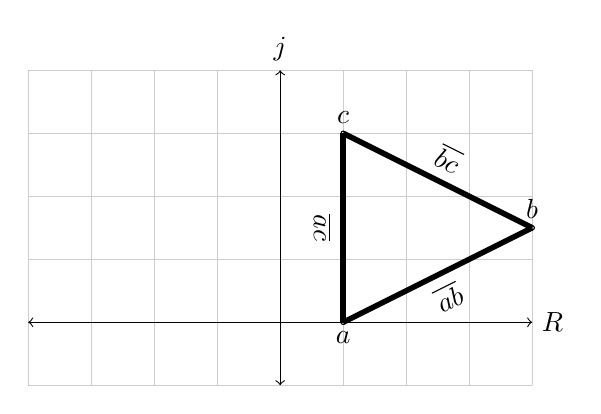
\begin{tikzpicture}[scale=0.8]
    \draw [thin,gray!40] (-4,-1) grid (4,4);
    \draw[<->] (-4,0)--(4,0) node[right] {$R$};
    \draw[<->] (0,-1)--(0,4) node[above]{$j$};
    \coordinate (a) at (1,0);
    \coordinate (b) at (4,1.5);
    \coordinate (c) at (1,3);
   
    \draw[black] (a) circle(1pt) node[anchor=north]{$a$};
    \draw[black] (b) circle(1pt) node[anchor=south]{$b$};
    \draw[black] (c) circle(1pt) node[anchor=south]{$c$};
    \draw[line width=2pt,black,-] (a)--(b) node[midway, below, sloped]{$\overline{ab}$};
    \draw[line width=2pt,black,-] (b)--(c) node[midway, above, sloped]{$\overline{bc}$};
    \draw[line width=2pt,black,-] (c)--(a) node[midway, below, sloped]{$\overline{ac}$};
\end{tikzpicture}
\caption*{Triangulo $s$}
    \end{minipage}
    \begin{minipage}{0.49\textwidth}
    \centering
        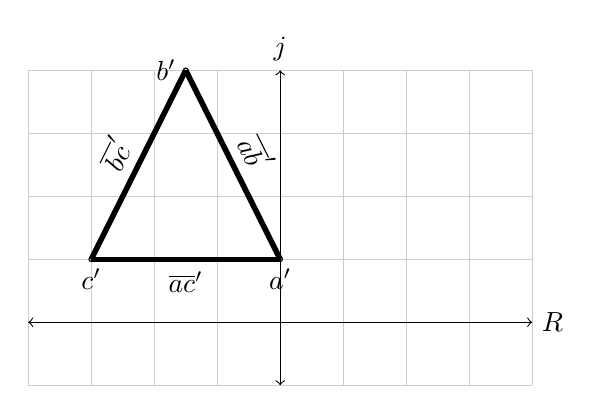
\begin{tikzpicture}[scale=0.8]
    \draw [thin,gray!40] (-4,-1) grid (4,4);
    \draw[<->] (-4,0)--(4,0) node[right] {$R$};
    \draw[<->] (0,-1)--(0,4) node[above]{$j$};
    \coordinate (1) at (0,1);
    \coordinate (2) at (-1.5,4);
    \coordinate (3) at (-3,1);
   
    \draw[black] (1) circle(1pt) node[anchor=north]{$a'$};
    \draw[black] (2) circle(1pt) node[anchor=east]{$b'$};
    \draw[black] (3) circle(1pt) node[anchor=north]{$c'$};
    \draw[line width=2pt,black,-] (1)--(2) node[midway, above, sloped]{$\overline{ab}'$};
    \draw[line width=2pt,black,-] (2)--(3) node[midway, above, sloped]{$\overline{bc}'$};
    \draw[line width=2pt,black,-] (3)--(1) node[midway, below, sloped]{$\overline{ac}'$};
\end{tikzpicture}
\caption*{Mapeo del triangulo $s$}
    \end{minipage}
    \caption{}
    \label{fig:RotF1}
\end{figure}
\begin{figure}[H]
    \centering
    \begin{tikzpicture}
    \draw [thin,gray!40] (-6,-2) grid (6,6);
    \draw[<->] (0,-2)--(0,6) node[anchor=south east]{$R'$};
    \draw[<->] (-6,0) node[left] {$j'$}--(6,0);
    \draw[mlgb,dashed] (-6,0)--(6,0) node[right] {$R$} ;
    \draw[mlgb,dashed] (0,-2)--(0,6) node[anchor=south west]{$j$};
    \coordinate (a) at (1,0);
    \coordinate (b) at (4,1.5);
    \coordinate (c) at (1,3);
    \coordinate (1) at (0,1);
    \coordinate (2) at (-1.5,4);
    \coordinate (3) at (-3,1);
   
    \draw[mlgb] (a) circle(1pt) node[anchor=north]{$a$};
    \draw[mlgb] (b) circle(1pt) node[anchor=south]{$b$};
    \draw[mlgb] (c) circle(1pt) node[anchor=south]{$c$};
    \draw[black] (1) circle(1pt) node[anchor=north]{$a'$};
    \draw[black] (2) circle(1pt) node[anchor=east]{$b'$};
    \draw[black] (3) circle(1pt) node[anchor=north]{$c'$};
    \draw[line width=1pt,mlgb,-] (a)--(b) node[midway, below, sloped]{$\overline{ab}$};
    \draw[line width=1pt,mlgb,-] (b)--(c) node[midway, above, sloped]{$\overline{bc}$};
    \draw[line width=1pt,mlgb,-] (c)--(a) node[midway, below, sloped]{$\overline{ac}$};
    \draw[line width=2pt,black,-] (1)--(2) node[midway, above, sloped]{$\overline{ab}'$};
    \draw[line width=2pt,black,-] (2)--(3) node[midway, above, sloped]{$\overline{bc}'$};
    \draw[line width=2pt,black,-] (3)--(1) node[midway, below, sloped]{$\overline{ac}'$};
    \draw[line width=1pt,black,dotted] (a) arc (0:90:1) ;
    \draw[line width=1pt,black,dotted] (b) arc (20.556:110.556:4.272) ;
    \draw[line width=1pt,black,dotted] (c) arc (71.565:161.565:3.1623) ;
    \draw[line width=1pt,black,dotted] (6,0) arc (0:90:6) ;
    \draw[line width=1pt,black,dashed] (0,6) arc (90:180:6) ;
\end{tikzpicture}
\caption{Plano $w$ graficado sobre el plano $z$ siendo $f_{z}$ un rotación}
    \label{fig:RotF3}
\end{figure}
\unsubsection{Funciones lineales}
Una función lineal es aquella que se describe como una suma de las funciones desplazamiento, escalado y dependiendo del factor de escalado una rotación. Se define una función lineal en un plano complejo como:
\begin{equation}
    w=f_{(z)}\lrah w=\lambda z+z_0
\end{equation}
Si $\lambda$ es un numero complejo, la ampliación con lleva una rotación. El mapeo de una curva entonces se puede realizar aplicando de forma progresiva las transformaciones. Primero la rotación, luego la ampliación y por ultimo el desplazamiento. Siempre se deben aplicar las transformaciones a las curvas afectadas por la ultima transformación. Se le por ejemplo plantemos el disco:
\begin{equation}
    \Vec{a}=re^{j\theta}+z_0\begin{cases}
        1\leq r\leq1.5\\
        z_0=(1+j0)
    \end{cases}
\end{equation}
\begin{figure}[H]
    \centering
    \begin{tikzpicture}[scale=0.7]
    \draw[thin,gray!40] (-4,-4) grid (4,4);
    \draw[<->] (-4,0)--(4,0) node[right] {$R$};
    \draw[<->] (0,-4)--(0,4) node[above]{$j$};
    \coordinate (a) at (1,0);
    \fill[fill=mlgb, fill opacity=0.6,even odd rule] (a) circle (1.5) (a) circle (1);
    \draw[fill=black] (a) circle(2pt) node[anchor=north east]{$z_0$};
    \draw [black,line width=2pt](a) circle (1);
    \draw [black,line width=2pt](a) circle (1.5);
\end{tikzpicture}
\caption{Disco en el plano complejo}
    \label{fig:LinF1}
\end{figure}
Y le aplicamos la transformación:
\begin{equation}
    w=f_(z)\lrah w=j2\cdot z-(-1+j)
\end{equation}
Entonces primero le aplicaríamos la rotación
\begin{equation}
    \vec{a}'=re^{j\theta}+j\begin{cases}
        1\leq r\leq1.5\\
    \end{cases}
\end{equation}
Como vemos, al ser un disco nuestra curva, la rotación solo afecto su centro. El argumento al estar acotado entre $pi$ y $-pi$, sumarle un $\frac{\pi}{2}$, correspondiente a la rotación, no con lleva afectar el modulo del intervalo, seguirá siendo un intervalo de modulo $2\pi$, entonces el disco seguirá siendo un disco completo. 

Luego le aplicamos la ampliación:
\begin{equation}
    \vec{\hat{a}}=2re^{j\theta}+2j\begin{cases}
        1\leq r\leq1.5\\
    \end{cases}
\end{equation}
Y por ultimo el desplazamiento:
\begin{equation}
     \vec{\hat{a}}'=2re^{j\theta}(1+j)\begin{cases}
        1\leq r\leq1.5\\
    \end{cases}
\end{equation}
\begin{figure}[H]
    \centering
    \begin{minipage}{0.29\textwidth}
    \centering
        \begin{tikzpicture}[scale=0.4]
    \draw[thin,gray!40] (-5,-5) grid (5,5);
    \draw[<->] (-5,0)--(5,0) node[right] {$R$};
    \draw[<->] (0,-5)--(0,5) node[above]{$j$};
    \coordinate (a) at (0,1);
    
    \fill[fill=mlgb, fill opacity=0.6,even odd rule] (a) circle (1.5) (a) circle (1);
    \draw[fill=black] (a) circle(2pt) node[anchor=north east]{$z_0$};
    \draw [black,line width=2pt](a) circle (1);
    \draw [black,line width=2pt](a) circle (1.5);
\end{tikzpicture}
\caption*{Rotación}

        \label{fig:LinRotF}
    \end{minipage}
    \begin{minipage}{0.29\textwidth}
    \centering
        \begin{tikzpicture}[scale=0.4]
    \draw[thin,gray!40] (-5,-5) grid (5,5);
    \draw[<->] (-5,0)--(5,0) node[right] {$R$};
    \draw[<->] (0,-5)--(0,5) node[above]{$j$};
    \coordinate (a) at (0,2);
    
    \fill[fill=mlgb, fill opacity=0.6,even odd rule] (a) circle (3) (a) circle (2);
    \draw[fill=black] (a) circle(2pt) node[anchor=north east]{$z_0$};
    \draw [black,line width=2pt](a) circle (2);
    \draw [black,line width=2pt](a) circle (3);
\end{tikzpicture}
\caption*{Ampliación}

        \label{fig:LinAmpF}
    \end{minipage}
    \begin{minipage}{0.29\textwidth}
    \centering
        \input{Plots/FuncionesComplejos/Mappeo/Lineal/LinF4}
        \label{fig:LinDesF}
    \end{minipage}
    \caption{}
\end{figure}
\begin{figure}[H]
    \centering
    \begin{tikzpicture}
    \coordinate (a) at (1,0);
    \draw[fill=mlgb] (a) circle(2pt) node[anchor=north west]{$z_0$};
    
    \draw[thin,mlgb] (-5,-5) grid (5,5);
    %\draw[step=2,line width=0.75pt,black] (-5,-5) grid (5,5);
    \draw[line width=0.75pt,black, dashed] (-5,0)--(5,0) node[right] {$R$};
    \draw[line width=0.75pt,black, dashed] (0,-5)--(0,5) node[above]{$j$};
    \draw[line width=1.5pt,<->] (-5,-1) node[left] {$j'$} --(5,-1) ;
    \draw[line width=1.5pt,<->] (1,-5)--(1,5) node[above]{$R'$};
    
    \coordinate (1) at (2,1);

    \fill[fill opacity=0.6, pattern=north east lines, pattern color=mlgb, even odd rule] (a) circle (1.5) (a) circle (1);
    
    \draw [mlgb,line width=1pt](a) circle (1);
    \draw [mlgb,line width=1pt](a) circle (1.5);
    
    \fill[fill=mlgb, fill opacity=0.6,even odd rule] (1) circle (3) (1) circle (2);
    \draw[fill=black] (1) circle(2pt) node[anchor=south west]{$z_0'$};
    \draw [black,line width=2pt](1) circle (2);
    \draw [black,line width=2pt](1) circle (3);
\end{tikzpicture}
\caption{Plano $w$ graficado sobre el plano $z$ siendo $f_{z}$ siendo una funcion lineal}
    \label{fig:}
\end{figure}

\unsubsection{Función reciproca}
La función reciproca se define como:
\begin{equation}
    w=\frac{1}{z}
\end{equation}
Esta es una transformación no lineal.
Plantemos una circunferencia genérica centrada en el origen:
\begin{equation}
\begin{aligned}
    &z_a=re^{j\theta}\begin{cases}
        r=\kappa\\
        -\pi<\theta\leq\pi
    \end{cases}
\end{aligned}
\end{equation}
Aplicándole la transformación obtenemos:
\begin{equation}
\begin{aligned}
     w_a=\frac{1}{z_a}\lrah &w_a=\frac{1}{re^{j\theta}}\lrah w_a=\frac{1}{r}e^{-j\theta}\begin{cases}
        r=\kappa\\
        -\pi<\theta\leq\pi
        \end{cases}
\end{aligned}
\end{equation}
Planteamos un cambio de variable:
\begin{equation}
\begin{aligned}
    \phi=-\theta \lrah -\pi<\theta\leq\pi&\\
                        -\pi<-\phi\leq\pi&\\
                        \pi>\phi\geq-\pi&
\end{aligned}
\end{equation}
Como vemos el argumento sigue existiendo en un intervalo de modulo $2\pi$, esto quiere decir que una función reciproca solo modifica el radio de la circunferencia. El radio $\kappa$ de una circunferencia en el plano complejo $z$ pasaría a ser de radio $\frac{1}{\kappa}$ en el plno complejo $w$. Se pueden denotar 3 casos distintos:
\begin{equation}
    \begin{cases}
        \kappa=1 \lrah \frac{1}{\kappa}=1\\
        \kappa\leq 1 \lrah \frac{1}{\kappa}\geq1\\
        \kappa\geq 1 \lrah \frac{1}{\kappa}\leq1
    \end{cases}
\end{equation}
Entonces a mayor radio en el plano $z$ menor sera el radio en $w$ siendo una circunferencia de radio uno el limite entre estas distintas regiones en el comportamiento.
\begin{figure}[H]
\centering
    \begin{minipage}{0.4\textwidth}
    \centering
       \begin{tikzpicture}[scale=0.7]
    \draw[thin,gray!40] (-4,-4) grid (4,4);
    \draw[<->] (-4,0)--(4,0) node[right] {$R$};
    \draw[<->] (0,-4)--(0,4) node[above]{$j$};
    \fill[fill=mlgb, fill opacity=0.6,even odd rule] (-4, -4) rectangle (4,4)(0, 0) circle (2);
    \draw [black,line width=2pt,fill=vorange,fill opacity=0.6](0, 0) circle (2);
    \draw[line width=1pt,|-|] (0,0) -- (2,0) node[midway,above,sloped]{$r=1$};
\end{tikzpicture}
\caption*{Regiones en el plano $z$}
    \label{fig:InvF1}
    \end{minipage}
    
   \begin{minipage}{0.4\textwidth}
    \centering
       \begin{tikzpicture}[scale=0.7]
    \draw[thin,gray!40] (-4,-4) grid (4,4);
    \draw[<->] (-4,0)--(4,0) node[right] {$R'$};
    \draw[<->] (0,-4)--(0,4) node[above]{$j'$};
    \path[fill=vorange, fill opacity=0.6,even odd rule] (-4, -4) rectangle (4,4) (0,0) circle (2);
    \draw [line width=2pt,black,fill=mlgb,fill opacity=0.6](0, 0) circle (2);
    \draw[line width=1pt,|-|] (0,0) -- (2,0) node[midway,above,sloped]{$r=1$};
\end{tikzpicture}
\caption*{Regiones en el plano $w$}
    \label{fig:InvF2}
    \end{minipage}
    \caption{}
    \label{fig:InvF}
\end{figure}
Esto se puede interpreta como que la función reciproca toma los puntos interiores del circulo unitario y los mapea en puntos exteriores al circulo unitario en el plano $w$ y viceversa.

Plantemos ahora una linea vertical, para ver como la función reciproca modifica la malla del plano $z$:
\begin{equation}
    z_a=\kappa+jy
\end{equation}
$\kappa$ siendo una constante.

Aplicándole la función reciproca se obtiene:
\begin{equation}
\begin{aligned}
      w_a=\frac{1}{z_a}\lrah w_a&=\frac{1}{\kappa+jy}\\
                             w_a&=\frac{1}{\kappa+jy}\cdot\frac{\kappa-jy}{\kappa-jy}\\
                              w_a&=\frac{\kappa-jy}{\kappa^2+y^2}\\
                               (u+jv)&=\underbrace{\frac{\kappa}{\kappa^2+y^2}}_\text{\clap{u~}}-j\underbrace{\frac{y}{\kappa^2+y^2}}_\text{\clap{v~}}\\
\end{aligned}
\end{equation}
Recordemos que la variable $w=u+jv$ entonces el mapeo de la recta estará dado por el sistema de ecuaciones:
\begin{equation}
    \begin{cases}
        u=\frac{\kappa}{\kappa^2+y^2}\\
        v=-\frac{y}{\kappa^2+y^2}
    \end{cases}
\end{equation}
Ambas ecuaciones son muy similares entre si, solo difieren en el numerador esto nos permite realizar un paso intermedio simple. Podes expresar $u$ en función de $v$ e $y$ para poder despejar la variable $y$.Luego aplicamos el método de sustitución y así eliminaremos una de nuestras variables dejando una función de 2 variables independientes. 
Vemos que:
\begin{equation}
     u=-\frac{v\kappa}{y} \lrah y=-\frac{v\kappa}{u}
\end{equation}
Resolviendo por sustitución en la ecuación $u=...$ :
\begin{equation}
    \begin{aligned}
        u=\frac{\kappa}{\kappa^2+y^2}\lrah &u=\frac{\kappa}{\kappa^2+(\cfrac{v\kappa}{u})^2}\lrah u=\frac{\kappa}{\kappa^2+\cfrac{v^2\kappa^2}{u^2}}\\
        &u=\frac{\bcancel{\kappa}}{\kappa^{\bcancel{2}}(1+\cfrac{v^2}{u^2})}\lrah u(1+\cfrac{v^2}{u^2})=\frac{1}{\kappa}\\
        &u+\cfrac{v^2}{u}=\cfrac{1}{\kappa}\lrah -v^2=(u-\cfrac{1}{\kappa})\cdot(u)\\
        &0=(u^2-\cfrac{u}{\kappa})+v^2\lrah\cfrac{1}{4\kappa^2}=(u^2-\cfrac{u}{\kappa}+\cfrac{1}{4\kappa^2})+v^2\\
        &(\cfrac{1}{2\kappa})^2=(u-\cfrac{1}{2\kappa})^2+v^2\\
        \label{eq:1/ZVer}
    \end{aligned}
\end{equation}
 Si recordamos la ecuación que describe una circunferencia en el plano de 2 dimensiones reales vemos que son prácticamente idénticas:
 \begin{equation}
     r^2=(x-x_0)^2+(y-y_0)^2
 \end{equation}
 Entones podemos afirmar que cualquier linea vertical desplazada en $\kappa$ sera mapeada en una circunferencia con centro $\frac{1}{2\kappa}$ sobre el eje real y de radio igual a su desplazamiento $r=\frac{1}{2\kappa}$. Al ser el modulo del radio igual al modulo del desplazamiento todas las circunferencias pasaran por el punto$(0,j0)$. 
\begin{figure}[H]
\centering
    \begin{minipage}{0.4\textwidth}
    \centering
       \input{Plots/FuncionesComplejos/Mappeo/Invers/InvF3}
    \end{minipage}
   \begin{minipage}{0.41\textwidth}
    \centering
       \begin{tikzpicture}
    \coordinate (a) at (1,0);
    \draw[thin,gray!40] (-2,-2) grid (2,2);
    
    \path[fill=mlgb, fill opacity=0.6,even odd rule] (0, -2) rectangle (2,2) (a) circle (1);
    \path [line width=2pt,black,fill=vorange,fill opacity=0.6](a) circle (1);
    
    \draw[<->] (-2,0)--(2,0) node[right] {$R$};
    \draw[<->] (0,-2)--(0,2) node[above]{$j$};
    
    
    \draw[line width=2pt] (1,0) circle(1);
    \draw[fill=black] (a) circle(2pt) node[below]{$\frac{1}{2\kappa}$};
    \draw[line width=1pt,black,|-|] (0,0)--(a) node[midway,above,sloped]{$\frac{1}{2\kappa}$};
\end{tikzpicture}
\caption*{Mapeo linea vertical}
    \end{minipage}
    \caption{}
    \label{fig:InvFV1}
\end{figure}
El mapeo para lineas horizontales es similar.
\begin{figure}[H]
\centering
    \begin{minipage}{0.4\textwidth}
    \centering
       \begin{tikzpicture}

    \draw[thin,gray!40] (-2,-2) grid (2,2);

    \path[draw=gray!40, fill=mlgb, fill opacity=0.6] (-2,1) -- (2,1) -- (2,0) -- (-2,0);
    \path[draw=gray!40, fill=vorange, fill opacity=0.6] (-2,1) -- (2,1) -- (2,2) -- (-2,2);
    
    \draw[<->] (-2,0)--(2,0) node[right] {$R$};
    \draw[<->] (0,-2)--(0,2) node[above]{$j$};
    
    \draw[fill=black] (0,1) circle(2pt) node[anchor=south east]{$\kappa$};
    \draw[line width=2pt,black,stealth-stealth] (-2,1)--(2,1) node[anchor=south west]{$(\kappa,jt)$};
\end{tikzpicture}
\caption*{Linea Horizontal}
    \end{minipage}
   \begin{minipage}{0.41\textwidth}
    \centering
       \input{Plots/FuncionesComplejos/Mappeo/Invers/InvF7}
    \end{minipage}
    \caption{}
    \label{fig:InvFV2}
\end{figure}
 Analizando la ecuación que rige el centro de la circunferencia vemos que a mayor distancia del la ordenada al origen en el plano $z$ menor va hacer su distancia a la ordenada al origen en el plano $w$ y menor va a ser su radio. Esto lo podemos relacionar con como, la función inversa, mapea a una circunferencia, ya que si en el plano $z$ la linea pasa por un punto $\kappa$ cercano a $0$ esta sera mapeada en una circunferencia de radio cercano a infinito, comportamiento que valida la idea que la función inversa mapea los puntos dentro de la circunferencia unitria fuera de este en el plano $w$. De todas maneras parte de los punto de la recta se siguen mapeando dentro de la circunferencia unitaria entonces la función reciproca más bien toma el plano $z$ y lo curva sobre la ordenada al origen en el infinito.
 \begin{figure}[H]
     \centering
     \begin{tikzpicture}
    \draw [thin,mlgb] (-6,-6) grid (6,6);
    \draw[mlgb,<->] (-6,0)--(6,0) node[anchor= north west] {$R$};
    \draw[mlgb,<->] (0,-6)--(0,6) node[anchor=south east]{$j$};
    \draw[<->] (-6,0)--(6,0) node[anchor=south west] {$R'$};
    \draw[<->] (0,6)--(0,-6) node[anchor=south west]{$j'$};
    \clip (-6,-6) rectangle (6,6);
    \foreach \c in {0.5,1,...,4.5} {
        \draw[line width=0.75pt,gray] (\c,0) circle(\c);
    }
    \foreach \c in {0.5,1,...,4.5} {
        \draw[line width=0.75pt,gray] (-\c,0) circle(\c);
    }
    \foreach \c in {0.5,1,...,4.5} {
        \draw[line width=0.75pt,gray] (0,\c) circle(\c);
    }
    \foreach \c in {0.5,1,...,4.5} {
        \draw[line width=0.75pt,gray] (0,-\c) circle(\c);
    }
    %\foreach \c in {1,2...,7} {
    %    \draw[line width=1pt,gray!40] (0,(1/(2\c))) circle((1/(2\c))^2);
    %}
    % \draw[line width=1pt] (0,0) circle(2);
    % \draw[line width=0.5pt,mlgb,dashed] (0,0) circle(2);
    % \draw[line width=0.5pt,blue,dashed] (0,0) circle(1);
    % \draw[line width=0.5pt,vorange,dashed] (0,0) circle(6);
    % \draw[line width=1pt,blue] (0,0) circle(4);
    % \draw[line width=1pt,vorange] (0,0) circle(0.6666);
    
    
\end{tikzpicture}
\caption{Plano $w$ graficado sobre el plano $z$ siendo $f_{z}$ un función reciproca}
 \end{figure}

En el caso del punto $(0,j0)$ la función reciproca es igual a $\infty$.

\unsubsection{Función potencia}
La función potencia se define como:
\begin{equation}
    w=z^n
\end{equation}
\unsubsubsection{Función $z^2$}
Planteando una circunferencia/arco genérico y una segmento de recta que pase por el punto $(0,j0)$:
\begin{equation}
    \begin{aligned}
        &z_a=re^{j\theta}\begin{cases}
            r=\kappa\\
            a\leq\theta\leq b
        \end{cases}\\
        \\
        &z_b=re^{j\theta}\begin{cases}
            c\leq r\leq d\\
            \theta=\kappa
        \end{cases}
    \end{aligned}
\end{equation}
Aplicándoles la función:
\begin{equation}
    w=z^2
\end{equation}
Obtenemos:
\begin{equation}
    \begin{aligned}
        &w_a={z_a}^2\lrah w_a=r^2e^{2j\theta}\begin{cases}
            r=\kappa\\
            a\leq\theta\leq b
        \end{cases}\\
        \\
        &w_b=z_b^2\lrah w_b=r^2e^{2j\theta}\begin{cases}
            a\leq r\leq\ b\\
            \theta=\kappa
        \end{cases}
    \end{aligned}
\end{equation}
Realizando cambios de variable $\phi=2\theta$ y $r'=r^2$ respectivamente:
\begin{equation}
\begin{cases}
    w_a=r^2e^{j\phi}\begin{cases}
            r=\kappa\\
            2a\leq\phi\leq 2b
        \end{cases}\\
    \\
    w_b=r'e^{2j\theta}\begin{cases}
        (a)^2\leq r'\leq\ b^2\\
        \theta=\kappa
        \end{cases}
\end{cases}
\end{equation}
Vemos que en el caso del arco $z_a$, la función $z^2$ extendió el rango de valores que podía tomar el argumento además de amplificar su radio. Si tuviéramos un circulo completo los limites del intervalo del argumento sobre pasarían el intervalo limite de $-\pi<\theta\leq\pi$. Podemos decir entonces que con un arco en $z$ podemos definir una circunferencia en el plano $w$. Esto lo podemos pensar como una dilatación del plano $z$, descripta en la figura \ref{fig:z^2F1}.

Y en el caso de la segmento de recta, se roto su argumento en $\theta$ y el intervalo de valores que pude tomar $r'$ son solo número4s reales positivos. Analizando los dominios, en el plno 
$z$ y $w$ de los módulos de semirrectas y segmentos:
\begin{equation}
    \begin{cases}
        0\leq r\leq\infty\lrah 0\leq r'\leq\infty\\
        -1\leq r\leq\ 2\lrah 1\leq r'\leq\ 4\\
        -3\leq r\leq\ 1\lrah 9\leq r'\leq\ 1\\
    \end{cases}
\end{equation}
Entonces podemos decir que la función $z^2$ mapea segmentos y semirrectas que no estén desplazadas en el plano $z$ en otros segmentos y semirrectas que posen un argumento de $2j\theta$. 


En el caso de la recta obtenemos un conflicto en el intervalo:
\begin{equation}
    \begin{cases}
        -\infty\leq r\leq\infty\lrah\infty\leq r'\leq\infty\\
    \end{cases}
\end{equation}
Para solucionar esta contradicción se puede construir una recta a partir de 2 semirrectas de modulo $0\leq r\leq\infty$ y de argumentos $j(\theta)$ y $j(\theta+\pi)$ para representar la parte positiva y negativa respectivamente. Aplicando la transformación vemos que los módulos de ambas semi rectas son iguales y los argumentos también. Recordando que $+2\pi$ en la expresión de un argumento equivale a una rotación de $360^{\circ}$:
\begin{equation}
    \begin{cases}
        j\theta\lrah j2\theta\\
        j(\theta+\pi)\lrah j(2\theta+2\pi)=j2\theta
    \end{cases}
\end{equation}
Una recta entonces se mapea en 2 semirrectas identicas.

\begin{figure}[H]
    \centering
    \begin{minipage} {0.49\textwidth}
    \centering
        \begin{tikzpicture}[scale=0.7]
    
    \foreach \ang in {0,...,31} {
        \draw [gray!40] (0,0) -- (\ang * 180 / 16:4);
    }
    \foreach \s in {0,0.5,...,3.5} {
        \draw [gray!40] (0,0) circle (\s);
    }
    \path[fill=mlgb, fill opacity=0.6] (0,0)--(4,0) arc(0:90:4) --(0,0);
    \path[fill=vorange, fill opacity=0.6] (0,0)--(4,0) arc(360:270:4)--(0,0);
    
    \draw[<->] (-4,0)--(4,0) node[right] {$R$};
    \draw[<->] (0,-4)--(0,4) node[above]{$j$};
    \draw [black,line width=0.5pt] circle (4);
    \draw[line width=0.75pt,mdrd,|-|] (0.3827*0.5,0.9239*0.5) arc (67.5:112.5:0.5);
    \draw[line width=0.75pt,mdblu,|-|] (0.3827,-0.9239) arc (-67.5:-112.5:1);
    \draw[line width=0.75pt,mblk,|-|] (-0.1951*1.5,0.9808*1.5) arc (101.25:168.75:1.5);
    
   % \path[fill opacity=0.6,pattern=dots,pattern color=mdblu, even odd rule] (0,0)--(0,4) arc(90:180:4)--(0,0);
   % \path[fill opacity=0.6,pattern=dots,pattern color=mdrd, even odd rule] (0,0)--(0,-4) arc(270:180:4)--(0,0);
\end{tikzpicture}
\caption*{Plano $z$}

    \end{minipage}
    \begin{minipage} {0.49\textwidth}
    \centering
        \begin{tikzpicture}[scale=0.7]
    \foreach \ang in {0,...,31} {
        \draw [gray!40] (0,0) -- (\ang * 360 / 16:4);
    }
    \foreach \s in {0.25,1,2.25,4} {
        \draw [gray!40] (0,0) circle (\s);
    }
    \path[fill=mlgb, fill opacity=0.6] (0,0)--(4,0) arc(0:180:4) --(0,0);
    \path[fill=vorange, fill opacity=0.6] (0,0)--(4,0) arc(360:180:4)--(0,0);
    
    \draw[<->] (-4,0)--(4,0) node[right] {$R$};
    \draw[<->] (0,-4)--(0,4) node[above]{$j$};
    \draw [black,line width=0.6pt] circle (4);
    \draw[line width=0.75pt,mblk,|-|] (-0.9239*2.25,-0.3827*2.25) arc (202.5:337.5:2.25);
    
    
    \draw[line width=0.75pt,mdrd,|-|] (-0.70711*0.25,0.70711*0.25) arc (135:225:0.25);
    \draw[line width=0.75pt,mdblu,|-|] (-0.70711,-0.70711) arc (-135:-225:1);

    
    %\path[fill opacity=0.6,pattern=dots,pattern color=mdblu,even odd rule] (0,0)--(4,0) arc(360:180:4)--(0,0);
    %\path[fill opacity=0.6,pattern=dots,pattern color=mdrd, even odd rule] (0,0)--(0,-4) (0,0)--(4,0) arc(0:180:4) --(0,0);
\end{tikzpicture}
\caption*{Plano $w$}

    \end{minipage}
    \caption{}
    \label{fig:z^2F1}
\end{figure}

Ahora que tenemos una idea de como afecta el plano complejo la función $z^2$, plantemos una recta vertical y horizontal para terminar de comprender como se modifica el espacio.
\begin{equation}
    \begin{cases}
        z_a=\kappa+jy\\
        z_b=x+j\kappa
    \end{cases}
\end{equation}
Aplicando la función $z^2$ a $z_a$:
\begin{equation}
    w_a={z_a}^2\lrah u+jv=\kappa^2-y^2+2jy\kappa
    \begin{cases}
        u=\kappa^2-y^2\\
        v=2y\kappa
    \end{cases}
\end{equation}
De la ecuación que describe $v$ podemos depejar la variable $y$ para luego resolver por sustitución.
\begin{equation}
    v=2y\kappa\lrah y=\frac{v}{2\kappa}
\end{equation}
\begin{equation}
\begin{aligned}
     u=\kappa^2-y^2\lrah &u=\kappa^2-(\frac{v}{2\kappa})^2\\
                        &(u-\kappa^2)=-\frac{v^2}{4\kappa^2}\\
                        \\
                        &(u-\kappa^2)4\kappa^2=-v^2
\end{aligned}
\end{equation}
Entonces una recta vertical centrada en $\kappa$ se mapea en una parábola de vértice $(\kappa^2,j0)$ y foco $\kappa^2$. Esto conlleva a que cualquier recta vertical se mapea en una parábola horizontal que abré hacia la izquierda y siempre tiene un vértice sobre el eje real positivo.
\begin{figure}[H]
    \centering
    \begin{minipage}{0.49\textwidth}
    \centering
        \begin{tikzpicture}
    \draw[thin,gray!40] (-3,-3) grid (3,3);
    \fill[fill=vorange, fill opacity=0.6,even odd rule] (-3,-3) rectangle (3,3) (1,-3) rectangle (2,3);
    \fill[fill=mlgb, fill opacity=0.6] (1,-3) rectangle (2,3);
    \draw[<->] (-3,0)--(3,0) node[right] {$R$};
    \draw[<->] (0,-3)--(0,3) node[above]{$j$};
    
    \draw[line width=2pt,black,stealth-stealth] (1,-3)--(1,3) node[midway, above left]{$\kappa_1$};
    \draw[line width=2pt,black,stealth-stealth] (2,-3)--(2,3) node[midway, above right]{$\kappa_2$};
\end{tikzpicture}
\caption*{Lineas verticales}
    \end{minipage}
    \begin{minipage}{0.49\textwidth}
    \centering
        \begin{tikzpicture}
        \draw[thin,gray!40] (-3,-3) grid (3,3);
        \path[rotate=90,opacity=0.6,fill=vorange,even odd rule] (-3,-3) rectangle (3,3) plot[smooth,domain=-2.55:2.55] (\x, {((\x)^2/1.3)-2}) plot[smooth,domain=-1.4142:1.4142] (\x, {((\x)^2*2)-1});
        \path[rotate=90,line width=2pt,fill=mlgb,fill opacity=0.6,even odd rule] plot[smooth,domain=-2.55:2.55] (\x, {((\x)^2/1.3)-2}) plot[smooth,domain=-1.4142:1.4142] (\x, {((\x)^2*2)-1});
        \draw[<->] (-3,0)--(3,0) node[right] {$R$};
        \draw[<->] (0,-3)--(0,3) node[above]{$j$};
        \draw[rotate=90,line width=2pt]   plot[smooth,domain=-2.55:2.55] (\x, {((\x)^2/1.3)-2}) (0,-2) node[above right]{$\kappa_2'$} plot[smooth,domain=-1.4142:1.4142] (\x, {((\x)^2*2)-1}) (0,-1) node[left]{$\kappa_1'$};
\end{tikzpicture}
\caption*{Plano complejo $w$}
    \end{minipage}
    \caption{}
    \label{fig:Z^2VF}
\end{figure}
Realizando el mismo procedimiento para las lineas horizontales obtenemos la ecuación:
\begin{equation}
    (u+\kappa^2)4\kappa^2=v^2
\end{equation}
A diferencia del mapeo para rectas verticales, el mapeo de rectas horizontales de como resultado parábolas horizontales que abren hacia la derecha y posen un vértice sobre el eje real negativo.
\begin{figure}[H]
    \centering
    \begin{minipage}{0.49\textwidth}
    \centering
        \begin{tikzpicture}
    \draw[thin,gray!40] (-3,-3) grid (3,3);
    \fill[fill=vorange, fill opacity=0.6,even odd rule] (-3,-3) rectangle (3,3) (-3,1) rectangle (3,2);
    \fill[fill=mlgb, fill opacity=0.6] (-3,1) rectangle (3,2);
    \draw[<->] (-3,0)--(3,0) node[right] {$R$};
    \draw[<->] (0,-3)--(0,3) node[above]{$j$};
    
    \draw[line width=2pt,black,stealth-stealth] (-3,1)--(3,1) node[midway, below right]{$\kappa_1$};
    \draw[line width=2pt,black,stealth-stealth] (-3,2)--(3,2) node[midway, above right]{$\kappa_2$};
\end{tikzpicture}
\caption*{Lineas horizontales}
    \end{minipage}
    \begin{minipage}{0.49\textwidth}
    \centering
        \input{Plots/FuncionesComplejos/Mappeo/Z^2/Z^2HF2}
    \end{minipage}
    \caption{}
    \label{fig:Z^2HF}
\end{figure}
Cabe aclarar que lo mostrado en las figuras \ref{fig:Z^2VF} y \ref{fig:Z^2HF} solo son una representación valida para cuando $\kappa_1$ y $\kappa_2$ son mayor a $1$. Si este no fuera el caso, se invertirían las posiciones relativas de $\kappa_1'$ y $\kappa_2'$.
\begin{figure}[H]
    \centering
    \begin{tikzpicture}
    \draw [thin,mlgb] (-6,-6) grid (6,6);
    \draw[mlgb,<->] (-6,0)--(6,0) node[anchor= south west] {$R$};
    \draw[mlgb,<->] (0,-6)--(0,6) node[anchor=south east]{$j$};
    \draw[<->] (0,0)--(6,0) node[anchor= north west] {$R'$};
    \draw[<->] (0,0)--(-6,0) node[anchor=south east]{$j'$};

    \foreach \c in {0.2,0.4,...,1} {
        \draw [rotate=90,gray] plot[smooth,domain=-(sqrt((6+\c^2)*(4*\c^2))):(sqrt((6+\c^2)*(4*\c^2)))](\x, {((\x)^2/(4*\c^2))-\c^2});
    }
    \foreach \c in {1.2,1.4,...,2.4} {
        \draw [rotate=90,gray] plot[smooth,domain=-6:6](\x, {((\x)^2/(4*\c^2))-\c^2});
    }

   \foreach \c in {0.2,0.4,...,1} {
        \draw [rotate=-90,gray] plot[smooth,domain=-(sqrt((6+\c^2)*(4*\c^2))):(sqrt((6+\c^2)*(4*\c^2)))](\x, {((\x)^2/(4*\c^2))-\c^2});
    }
    \foreach \c in {1.2,1.4,...,2.4} {
        \draw [rotate=-90,gray] plot[smooth,domain=-6:6](\x, {((\x)^2/(4*\c^2))-\c^2});
    }
\end{tikzpicture}
\caption{Plano $w$ graficado sobre el plano $z$ siendo $f_{z}$ un función $z^2$}
    \label{fig:Z^2FC}
\end{figure}
\unsubsubsection{Función $z^{1/2}$}
La función $z^{1/2}$ al ser la inversa de la función $z^2$ genera el efecto contrario, contrayendo el espacio $z$, en su totalidad, en los cuadrantes $1$ y $4$ en el plano $w$.
Planteando una arco/circunferencia genérica que tengan por centro el punto $(0,j0)$ y una recta que pase por ese mismo, vemos que sus mapeos respectivos son entonces:
\begin{equation}
    \begin{aligned}
        &w_a={z_a}^{\cfrac{1}{2}}\lrah w_a=\sqrt{r}e^{j\frac{\theta}{2}}\begin{cases}
            r=\kappa\\
            -a\leq\theta\leq b
        \end{cases}\\
        \\
        &w_b=z_b^{\cfrac{1}{2}}\lrah w_b=\sqrt{r}e^{j\frac{\theta}{2}}\begin{cases}
            a\leq r\leq\ b\\
            \theta=\kappa
        \end{cases}
    \end{aligned}
\end{equation}
Realizando cambios de variable $\phi=\frac{\theta}{2}$ y $r'=\sqrt{r}$ respectivamente:
\begin{equation}
\begin{cases}
    w_a=\sqrt{r}e^{j\phi}\begin{cases}
            r=\kappa\\
            -\frac{a}{2}\leq\phi\leq \frac{b}{2}
        \end{cases}\\
    \\
    w_b=r'e^{j\frac{\theta}{2}}\begin{cases}
        \sqrt{a}\leq r'\leq\ \sqrt{b}\\
        \theta=\kappa
        \end{cases}
\end{cases}
\end{equation}
Se pude apreciar como se reduce el tamaño del intervalo para las variables independientes. Esto se puede interpretar como una contracción del espacio, expresado en la figura \ref{fig:z^0.5F1}.
\begin{figure}[H]
    \centering
    \begin{minipage}{0.49\textwidth}
    \centering
        \input{Plots/FuncionesComplejos/Mappeo/z^0.5/z^0.5F1}
    \end{minipage}
    \begin{minipage}{0.49\textwidth}
    \centering
        \begin{tikzpicture}[scale=0.7]
    
    \foreach \ang in {0,0.5,1,...,31} {
        \draw [gray!40] (0,0) -- (\ang * 180 / 16:4);
    }
    \foreach \s in {0,0.25,0.5,...,4} {
        \draw [gray!40] (0,0) circle (\s);
    }
    \draw[line width=0.5,black,fill=mlgb, fill opacity=0.6] (0,0)--(4,0) arc(0:45:4) --(0,0);
    \draw[line width=0.5,black,fill=vorange, fill opacity=0.6] (0,0)--(4,0) arc(360:315:4)--(0,0);
    
    \draw[<->] (-4,0)--(4,0) node[right] {$R$};
    \draw[<->] (0,-4)--(0,4) node[above]{$j$};
    \draw [black,line width=0.5pt] circle (4);
    \draw[line width=0.75pt,mdrd,|-|] (0.966*1.732,0.259*1.732) arc (15:75:1.732);
    \draw[line width=0.75pt,mdblu,|-|] (0.999,-0.0436) arc (-2.5:-42.5:1);
    
   % \path[fill opacity=0.6,pattern=dots,pattern color=mdblu, even odd rule] (0,0)--(0,4) arc(90:180:4)--(0,0);
   % \path[fill opacity=0.6,pattern=dots,pattern color=mdrd, even odd rule] (0,0)--(0,-4) arc(270:180:4)--(0,0);
\end{tikzpicture}
\caption*{Plano $z$}
    \end{minipage}
    \caption{}
    \label{fig:z^0.5F1}
\end{figure}
En el caso de las lineas verticales y horizontales su mapeo es complicado en el análisis ya que si planteamos dos lineas arbitrarias perpendiculares entre ellas:
\begin{equation}
    \begin{aligned}
    &z_a=\kappa_1+jy\\
    &z_b=x+j\kappa_2
    \end{aligned}
\end{equation}
Y le aplicamos la transformación $z^{1/2}$ obtenemos los siguientes sistemas de ecuaciones:
\begin{equation}
    \begin{aligned}
    &w_a=\begin{cases}u^2-v^2=\kappa_1\\2uv=y\end{cases}\\
    &w_b=\begin{cases}u^2-v^2=x\\2uv=\kappa_2\end{cases}
    \end{aligned}
\end{equation}
Estas ecuaciones son difícilmente graficables ya que dan como resultado una ecuación de 3 incógnitas para un plano de 2 dimensiones.
Expresando las rectas verticales y horizontales utilizando la forma polar, podríamos ser capaces de solucionar esta situación:
\begin{equation}
    \begin{aligned}
        &z_a=\sqrt{\kappa_1^2+y^2}\hspace{0.2cm}e^{j\frac{\arctan{(y/\kappa_1)}}{2}}\\
        &\\
        &z_b=\sqrt{x^2+\kappa_2^2}\hspace{0.2cm}e^{j\frac{\arctan{(\kappa_2/x)}}{2}}
    \end{aligned}
\end{equation}
Aplicando la función $z^{1/2}$ y expresando la incógnita $w$ en su forma polar $r_we^{j\phi}$ obtenemos los siguientes sistemas de ecuaciones:
\begin{equation}
\begin{aligned}
    &\begin{cases}
        r_{wa}=\sqrt{\sqrt{\kappa_1^2+y^2}}\\
        \phi_{wa}=\arctan{(y/\kappa_1)}{2}
    \end{cases}
    &\\
    &\\
    &\begin{cases}
        r_{wb}=\sqrt{\sqrt{x^2+\kappa_2^2}}\\
        \phi_{wb}=\arctan{(\kappa_2/x)}{2}
    \end{cases}
\end{aligned}
\end{equation}
Resolviendo el primer sistema de ecuaciones:
\begin{equation}
    \phi_{wa}=\arctan{y/\kappa_1}{2}\lrah y=\tan{(2\phi_{wa})}\cdot\kappa_1
\end{equation}
\begin{equation}
    r_{wa}=\sqrt{\kappa_1^2+y^2}\lrah r_{wa}=\sqrt{\kappa_1\sqrt{1+(\tan{(2\phi_{wa})})^2}}
\end{equation}
\begin{equation}
    \begin{aligned}
        w_a=&r_{wa}e^{j\phi}\\
        w_a=&\sqrt{\kappa_1\sqrt{1+(\tan{(2\phi_{wa})})^2}}\hspace{0.2cm}e^{j\phi}
    \end{aligned}
\end{equation}
Observemos que los valores posible para $\arctan{(y/\kappa_1)}$ están dentro del intervalo $-\pi<\arctan{(y/\kappa_1)}\leq\pi$, por lo tanto $\frac{\pi}{2}<\phi\leq\frac{\pi}{2}$.
En el caso de las lineas verticales obtenemos:
\begin{equation}
    \begin{aligned}
        w_b=&r_{wb}e^{j\phi}\\
        w_b=&\sqrt{\sqrt{\kappa_2^2+\frac{1}{\tan{(2\phi_{wa})}\cdot\kappa_2)^2}}} \hspace{0.2cm}e^{j\phi}
    \end{aligned}
\end{equation}
Se utilizo un software externo para aproximar las transformaciones de las lineas verticales (Azul) y horizontales (Rojo).
\begin{figure}[H]
    \centering
    %\includegraphics[height=15cm,trim=13cm 2cm 17cm 0,clip]{Imagenes/Z^0.5.pdf}
    \caption{Plano $w$ graficado sobre el plano $z$ siendo $f_{z}$ una función $z^{1/2}$}
    \label{fig:z^0.5cf}
\end{figure}
\unsubsection{Función logaritmo natural}
La función logaritmo natural se define como:
\begin{equation}
    w=\ln{(z)}
\end{equation}
Si recordamos como es la definición del operador logaritmo natural \ref{eq:defLnC} resulta evidente que semirrectas positivas que pasen por el origen serán transformadas en lineas horizontales que pase por el punto$(0,j\theta)$  , ya que las rectas se definen utilizando un argumento constante.
\begin{equation}
    z_a=re^{j\theta}\begin{cases}
        a\leq r\leq b\\
        \theta=\kappa
    \end{cases}
\end{equation}
Transformando:
\begin{equation}
    w_a=\ln{(z_a)}\lrah w_a=\ln{(r)}+j\theta\begin{cases}
        a\leq r\leq b\\
        \theta=\kappa
    \end{cases}
\end{equation}
Recordemos que el limite $\lim_{r\to\infty}\ln{(r)}=\infty$ y que $\lim_{r\to 0}\ln{(r)}=-\infty$. 
Para el caso de rectas, ya que para números negativos, la función $\ln{(x)}
$ no esta definida, para poder saber que sucede en el caso de los números negativos que puede tomar $r$ utilizaremos la misma técnica de construir una recta con 2 semirrectas que utilizamos para la función $z^2$.
\begin{equation}
    z_a=re^{j\theta}\begin{cases}
        -a\leq r\leq b\\
        \theta=\kappa
        \end{cases}\lrah\begin{cases}
            z_1=re^{j\theta}\begin{cases}
                0\leq r\leq b\\
            \end{cases}\\
            \\
            z_2=re^{j(\theta+\pi)}\begin{cases}
                a\leq r< 0\\
            \end{cases}
        \end{cases}
\end{equation}
Entonces para el caso de $z_2$ el mapeo sera igual a:
\begin{equation}
    w_2=\ln{(z_2)}\lrah w_2=\ln{(r)}+j(\theta+\pi)
\end{equation}
Vemos que la semirrecta negativa se mapea en otra linea horizontal que pasa por el punto $(0,j(\theta+\pi))$ o el punto $(0,j((\theta+\pi)-2\pi))$ este ultimo sea el caso en el cual el argumento se mayor que $2\pi$. Además la ordenada al origen siempre estará acotada entre $-\pi$ y $\pi$.
\begin{figure}[H]
    \centering
    \begin{minipage}{0.49\textwidth}
        \centering
        \begin{tikzpicture}
    \draw[thin,gray!40] (-3,-3) grid (3,3);
    \draw[<->] (-3,0)--(3,0) node[right] {$R$};
    \draw[<->] (0,-3)--(0,3) node[above]{$j$};
    
    \draw[line width=2pt,black,stealth-stealth] (-3,-3)--(0,0) ;
    \draw[line width=2pt,black,stealth-stealth] (0,0)--(3,3) ;
    \draw[line width=1pt,black,|-|] (1,0) arc (0:45:1) node [midway,left]{$\theta$};
    \draw[line width=1pt,black,|-|] (1,0) arc (0:-135:1) node [midway, above]{$\phi$};
\end{tikzpicture}
\caption*{Plano $z$}
    \end{minipage}
    \begin{minipage}{0.49\textwidth}
        \centering
        \begin{tikzpicture}
    \draw[thin,gray!40] (-3,-3) grid (3,3);
    \draw[<->] (-3,0)--(3,0) node[right] {$R$};
    \draw[<->] (0,-3)--(0,3) node[above]{$j$};
    
    \draw[line width=2pt,black,stealth-stealth] (-3,2)--(3,2)  node [midway,anchor=south west]{$\theta$};
    \draw[line width=2pt,black,stealth-stealth] (-3,-2)--(3,-2) node [midway,anchor=south west]{$\phi$};
\end{tikzpicture}
\caption*{Plano $w$}
    \end{minipage}
    \caption{}
    \label{fig:LnF1}
\end{figure}
El mapeo de las circunferencias y arcos es justo contrario al de rectas y semirrectas, al estar definidas por un modulo constante y un argumento variable serán mapeadas en lineas verticales.
\begin{equation}
   z_b=re^{j\theta}\begin{cases}
        r=\kappa\\
        a\leq\theta\leq b
   \end{cases} 
\end{equation}
Transformando:
\begin{equation}
    w_b=\ln{(z_b)}\lrah w_b=\ln{(r)}+j\theta\begin{cases}
        r=\kappa\\
        a\leq\theta\leq b
    \end{cases}
\end{equation}
Las lineas verticales en el plano $w$ que sean un mapeo de una circunferencia o un arco siempre estarán acotadas entre $\pi$ y $-\pi$ por como se define una circunferencia.
\begin{figure}[H]
    \centering
    \begin{minipage}{0.49\textwidth}
        \centering
        \begin{tikzpicture}
    \draw[thin,gray!40] (-3,-3) grid (3,3);
    \path[fill=vorange,fill opacity=0.6,even odd rule] (-3,-3) rectangle (3,3) (0,0) circle(1);
    \path[line width=2pt,black,dashed, fill=mlgb,fill opacity=0.6] (0,0) circle(1);
    
    \draw[<->] (-3,0)--(3,0) node[right] {$R$};
    \draw[<->] (0,-3)--(0,3) node[above]{$j$};
    \draw[line width=2pt,black,dashed] (0,0) circle(1);
    \draw[line width=1pt,black,|-|](0,0)--(1,0)node[midway,below]{$1$};
    \draw[line width=2pt,black,|-|] (0.7071*2,0.7071*2) arc(45:-45:2);
    \draw[line width=1pt,black,|-|](0,0)--(0.8192*2,0.5735*2)node[midway,above right,sloped]{$r$};
    
\end{tikzpicture}
\caption*{Plano $z$}
    \end{minipage}
    \begin{minipage}{0.49\textwidth}
        \centering
        \begin{tikzpicture}
    \draw[thin,gray!40] (-3,-3) grid (3,3);
    \path[fill=mlgb,fill opacity=0.6] (-3,-3) rectangle (0,3);
    \path[fill=vorange,fill opacity=0.6] (3,3) rectangle (0,-3);
    
    \draw[<->] (-3,0)--(3,0) node[right] {$R$};
    \draw[<->] (0,-3)node [anchor=south east]{$-\pi$}--(0,3) node[above]{$j$} node [anchor=north east]{$\pi$};
    \draw[line width=2pt,black,|-|] (1,-1.5)--(1,1.5) node[midway, anchor=south west]{$\ln{(r)}$};
    \draw[line width=2.5pt,black,dashed] (0,-3)--(0,3);

   
\end{tikzpicture}
\caption*{Plano $w$}
    \end{minipage}
    \caption{}
    \label{fig:LnF2}
\end{figure}
Para el caso de las lineas verticales y horizontales utilizaremos el mismo método que se utilizo para la función $z^{1/2}$.
Expresando las lineas en su forma polar:
\begin{equation}
    \begin{aligned}
        &z_a=\sqrt{\kappa_1^2+y^2}\hspace{0.2cm}e^{j\arctan{(y/\kappa_1)}}\\
        &\\
        &z_b=\sqrt{x^2+\kappa_2^2}\hspace{0.2cm}e^{j\frac{\arctan{(\kappa_2/x)}}{2}}
    \end{aligned}
\end{equation}
Aplicando la función $\ln{(z)}$ a $z_a$ obtenemos:
\begin{equation}
    w_a=\ln{(z_a)}\lrah w_a=\ln{(\sqrt{\kappa_1^2+y^2})}+j\arctan{(y/\kappa_1)}
\end{equation}
Entonces el mapeo estar dado por el siguiente sistema de ecuaciones:
\begin{equation}
    w_a\begin{cases}
        u=\ln{(\sqrt{\kappa_1^2+y^2})}
        v=\arctan{(y/\kappa_1)}
    \end{cases}
\end{equation}
Expresando $y$ en función de $v$:
\begin{equation}
    v=\arctan{(y/\kappa_1)}\lrah\tan{(v)}\cdot\kappa_1=y
\end{equation}
Y resolviendo por sustitución en $u$:
\begin{equation}
    \begin{aligned}
         u=\ln{(\sqrt{\kappa_1^2+y^2})}\lrah &u=\ln{(\sqrt{\kappa_1^2+(\tan{(v)}\cdot\kappa_1)^2})}\\
                                            &u=\ln{(\kappa_1\sqrt{1+\tan{(v)}^2})}\\
                                            &u=\ln{(\kappa_1)}+\ln{(\sqrt{1+\tan{(v)}^2})}
    \end{aligned}
\end{equation}
En el caso de las lineas horizontales el mapeo es igual a :
\begin{equation}
    u=\ln{(\kappa_2)}+\ln{(\sqrt{1+\frac{1}{\tan{(v)}^2}})}
\end{equation}
\begin{figure}[H]
    \centering
    \input{Plots/FuncionesComplejos/Mappeo/LogNa/LnCF}
    \caption*{}
    \label{fig:enter-label}
\end{figure}

\unsection{Función bilineal}
Una función bilineal es una conjunción de las funciones de desplazamiento, ampliación y reciproca y suele ser de la forma:
\begin{equation}
    w=\frac{a\cdot z+b}{c\cdot z+d}
    \label{eq:DefBil}
\end{equation}
Siendo $a$, $b$, $c$ y $d$ constantes.
Una función bilineal, al ser una construcción de otras funciones, se puede separar en distintas transformaciones.

Si realizamos una división de polinomios:
\begin{equation}
    \begin{array}{*1r @{\hskip\arraycolsep}c@{\hskip\arraycolsep} *{11}r}
        az+b &  &|\underline{cz+d}  \\
        -az-\frac{ad}{c}&        & \frac{a}{c}\\[5pt]
        \cline{1-1}
        b-\frac{ab}{c}    &          &    \\[-5pt]
\end{array}
\end{equation}
Entonces:
\begin{equation}
    az+b=\frac{a}{c}(cz+d)+(b-\frac{ab}{c})
    \label{eq:Bil1}
\end{equation}
Si remplazamos \ref{eq:Bil1} en \ref{eq:DefBil}
\begin{equation}
\begin{aligned}
    w=\frac{a\cdot z+b}{c\cdot z+d}\lrah W=&\cfrac{\frac{a}{c}(cz+d)+(b-\frac{ab}{c})}{c\cdot z+d}\\
                                          =&\cfrac{a}{c}+\cfrac{(b-\cfrac{ab}{c})}{c}\cdot\cfrac{1}{z+\frac{d}{c}}                          
\end{aligned}
\end{equation}
Al ser $a$, $b$, $c$ y $d$ constantes los términos $\frac{a}{c}$ y $\frac{d}{c}$ son desplazamientos por y el termino $\frac{(b-\frac{ab}{c})}{c}$ es una ampliación, asignando $z_0$, $z_1$ y $\kappa$ a cada uno de los términos obtenemos:
\begin{equation}
    w=z_0+\kappa\cfrac{1}{z+z_1}
\end{equation}
Entonces para computar el mapeo primero realizaremos el desplazamiento en $z_1$ luego seguiría la función reciproca, después la ampliación en $\kappa$ y por ultimo el desplazamiento en $z_0$.
Planteando una función bilineal cualquiera:
\begin{equation}
    f_{(z)}=\frac{3z+j2}{z}
\end{equation}
Podemos fácilmente separar los elementos que componen esta bilineal.
\begin{equation}
    f_{(z)}=3+2j\frac{1}{z}
\end{equation}
En este caso la ampliación conlleva también una rotación. Planteando un numero complejo en su forma exponencial para cubrir como se mapean circunferencias y rectas que pasen por el origen:
\begin{equation}
    w=3+2j\cfrac{1}{re^{j\theta}}\lrah 2=3+\frac{2}{r}e^{j(\pi-\theta)}
\end{equation}
En el caso que queramos representar un arco:
\begin{equation}
    z=re^{j\theta}\begin{cases}
        r=2\\
        -\frac{\pi}{3}\leq\theta\leq\frac{2\pi}{3}
    \end{cases}
\end{equation}
Este sera mapeado en otro arco de radio $r=1$, con centro en $(3,j0)$ y argumento de $\frac{\pi}{3}\leq\theta\leq\frac{4\pi}{3}$.
Casos en el que tengamos un desplazamiento en el numerador es recomendable plantearlo de manera gráfica, para luego realizar un análisis mas detallado,  por ejemplo sea una transformación bilineal de la forma:
\begin{equation}
    f_{(z)}=\cfrac{3z+2}{z+3}
\end{equation}
Realizando la división nos queda:
\begin{equation}
    w=\cfrac{3(z+3)-7}{z+3}\lrah w=3-7\cfrac{1}{z+3}
\end{equation}
Y queremos mapear una linea vertical que pase por el punto $(2,j0)$. Gráficamente podemos plantear 4 planos distintos en los cuales se apliquen las transformaciones de forma progresiva.
\begin{figure}[H]
    \centering
    \begin{tikzpicture}[node distance=4.5cm,thick,auto,main node/.style={rectangle,draw}]
    \node[main node] (1) {Plano $z$};
    \node[main node] (2) [below of=1] {Plano $\gamma$};
    \node[main node] (3) [right of=2] {Plano $\tau$};
    \node[main node] (4) [right of=3] {Plano $\lambda$};
    \node[main node] (5) [above of=4] {Plano $w$};
    \path[every node/.style={font=\sffamily\small}];
    \draw[-latex]
    (1) edge  node {Traslación $z_1$} (2)
        edge  node {$F_{(z)=}z_0+\kappa\cfrac{1}{z+z_1}$} (5)
    (2) edge  node {Reciproca $\frac{1}{z}$} (3)
    (3) edge  node {Escalado $\kappa$} (4)
    (4) edge  node[right] {Traslación $z_0$} (5);
\end{tikzpicture}
    \caption{Diagrama de flujo de una mapeo bilineal}
    \label{fig:DiagBil}
\end{figure}
La linea primero es desplazada por $z_1=3$, haciendo que ahora pase por el punto $(5,j0)$, sabiendo como se comporta la función reciproca de la ecuación \ref{eq:1/ZVer} sabemos que esta linea vertical sera transformada en una circunferencia de centro $(\frac{1}{10},j0)$ y de radio $r=\frac{1}{10}$, luego esta circunferencia es ampliada en un factor $\kappa=-7$ llevando el centro a $(-\frac{7}{10},j0)$  y el radio a $r=\frac{7}{10}$ y por ultimo un desplazamiento $z_0=3$ llevando el centro de la circunferencia a $(\frac{23}{10})$.
\begin{figure}[H]
    \centering
    \begin{minipage}{0.49\textwidth}
        \centering
        \begin{tikzpicture}
    \draw[thin,gray!40] (-3,-3) grid (3,3);
    \draw[<->] (-3,0)--(3,0) node[right] {$R$};
    \draw[<->] (0,-3)--(0,3) node[above]{$j$};
    \draw[line width=2pt, black,stealth-stealth] (3,-3)--(3,3) node[midway,anchor=south east]{$(5,j0)$};
    
\end{tikzpicture}
\caption*{Plano $\gamma$}
    \end{minipage}
    \begin{minipage}{0.49\textwidth}
        \centering
        \begin{tikzpicture}
    \draw[step=2.0,thin,gray!40] (-3,-3) grid (3,3);
    \draw[<->] (-3,0)--(3,0) node[right] {$R$};
    \draw[<->] (0,-3)--(0,3) node[above]{$j$};
    
    \draw[line width=2pt,black,-] (0.2,0) circle(0.2);
    
\end{tikzpicture}
\caption*{Plano $\tau$}
    \end{minipage}
    \begin{minipage}{0.49\textwidth}
        \centering
        \input{Plots/FuncionesComplejos/Mappeo/Bilineal/BilF3}
    \end{minipage}
    \begin{minipage}{0.49\textwidth}
        \centering
        \begin{tikzpicture}
    \draw[step=1.7,thin,gray!40] (-3,-3) grid (3,3);
    \draw[<->] (-3,0)--(3,0) node[right] {$R$};
    \draw[<->] (0,-3)--(0,3) node[above]{$j$};
    \draw[line width=2pt,black,-] (2.3,0) circle(0.7);

\end{tikzpicture}
\caption*{Plano $W$}
    \end{minipage}
    \caption{Aplicación método gráfico}
    \label{fig:TransBil}
\end{figure}

\unsection{Funciones como campos vectoriales}
Una función compleja se puede representar también como un campo vectorial, tomando una función cualquiera $f_{(x,jy)}=u+jv$ podemos representar la transformación del pano $z$ a través de vectores que tengan por punto de origen $(x,jy)$ y por punto final la suma entre el punto de origen y el punto transformado $w$ siendo esto igual a $(x+u,j(y+v))$.Para estas representaciones gráficas se separar la información en 2 gráficos distintos, un campo vectorial normalizado (quiere decir que a cada vector resultante se lo divide por su propia magnitud dejando un vector de modulo $=1$) solo útil para ver la dirección en la que se mapea el punto $(x,jy)$ y un campo escalar con el valor del modulo de los vectores, este ultimo se lo suele representar con colores o en un gráfico tridimensional siendo el eje $"z"$ representante de la magnitud del vector.

Un ejemplo seria el de la función $\frac{1}{z}$, de las secciones anteriores sabemos que a medida que el punto $(x,jy)$ este mas cercano al origen del plano $z$ mas lejos sera mapeado en el plano $w$ y viceversa. Tomemos el ejemplo del punto $(0.1,j0.1)$, pasándolo a su forma exponencial obtenemos $0.1414...e^{j\frac{\pi}{4}}$, y aplicando la función reciproca obtenemos el punto mapeado estará en $7.07e^{-j\frac{\pi}{4}}=(5,-j5)$. Entonces en la representación vectorial el vector asociado al punto $(0.1,j0.1)$ se extenderá desde el punto $(0.1,j0.1)$ al punto $(5.1,j-4.9)$ que normalizándolo seria $(0.721,-j0.65)$ y en el campo escalar en el punto $(0.1,j0.1)$ la ordenada a $z$ seria igual a $7.07$ que es el valor del modulo del vector sin normalizar.


\begin{figure}[H]
    \centering
    \begin{minipage}{0.49\textwidth}
        \centering
        %\input{Plots/FuncionesComplejos/VectFil/InvVectF1}
    \end{minipage}
    \begin{minipage}{0.49\textwidth}
        \centering
        %\begin{tikzpicture}
\begin{axis}[
 view={110}{30},
    unbounded coords=jump,
    z filter/.expression={
        z>20 ? nan : z
    }
]
\addplot3[surf,]{sqrt((-x/(x^2+y^2))^2+(y/(x^2+y^2))^2)};
\end{axis}
\end{tikzpicture}
\caption*{Campo escalar del modulo}
    \end{minipage}
    \caption{Representacion vectorial de la función $1/z$}
    \label{fig:VectFInvz}
\end{figure}
\begin{figure}[H]
    \centering
    \begin{minipage}{0.49\textwidth}
        \centering
        %\begin{tikzpicture}
\begin{axis}[
view = {0}{90},
%unbounded coords=jump,
   % x filter/.expression={
   %     x>9 ? nan : x
   % },
%unbounded coords=jump,
  %  y filter/.expression={
   %     y>9 ? nan : y
  %  }
]
\addplot3[
        quiver = {
                u = {(x^2-y^2)/sqrt((x^2-y^2)^2+(2*x*y)^2)},
                v = {(2*x*y)/sqrt((x^2-y^2)^2+(2*x*y)^2)},
            scale arrows = 0.4},
            domain = -5:5,
            domain y = -5:5,
        -stealth] {0};
\end{axis}
\end{tikzpicture}
\caption*{Representación vectorial normalizada}
    \end{minipage}
    \begin{minipage}{0.49\textwidth}
        \centering
        %\input{Plots/FuncionesComplejos/VectFil/z^2EscF1}
    \end{minipage}
    \caption{Representacion vectorial de la función $z^2$}
    \label{fig:VectFZ^2}
\end{figure}
\unsubsection{Poly-vector field}
Si se aplica el operador de conjugación sobre las representaciones vectoriales de las funciones complejas se obtiene lo que se denomina un campo poly-vectorial que forman patrones de flujo en campos en los cuales existe una "singularidad":
\begin{figure}[H]
    \centering
    %\input{Plots/FuncionesComplejos/VectFil/InvPloyVect}
    \caption{Poly-vector field de la función 1/z}
    \label{inv-Poly-vector}
\end{figure}
\begin{figure}[H]
    \centering
    \input{Plots/FuncionesComplejos/VectFil/z^2PolyVect}
    \caption{Poly-vector field de la función 1/z}
    \label{z^2-Poly-vector}
\end{figure}

\end{document}
